% arara: pdflatex
% arara: biber
% arara: pdflatex

\documentclass[11pt,a4paper,headsepline,bibliography=totoc,idxtotoc,DIV12,openright,twoside=true,chapterprefix=on]{scrbook}
%draft zum Schluss
\listfiles

\renewcommand*{\chapterheadstartvskip}{\vspace*{5cm}} %rausnehmen scrbook
%\pagestyle{myheadings}
%\markright{Basics}

\addtokomafont{pageheadfoot}{\linespread{1}\selectfont}
\usepackage[rflt]{floatflt}
\usepackage[german]{babel}
\usepackage{siunitx}
\usepackage{color}

\usepackage{xcolor}
\usepackage{listings}
\usepackage{bera}% optional; just for the example
\colorlet{punct}{red!60!black}
\definecolor{background}{HTML}{EEEEEE}
\definecolor{delim}{RGB}{20,105,176}
\colorlet{numb}{magenta!60!black}

\lstdefinelanguage{json}{
    basicstyle=\tiny\ttfamily,
    numbers=left,
    numberstyle=\scriptsize,
    stepnumber=1,
    numbersep=8pt,
    showstringspaces=false,
    breaklines=true,
    frame=lines,
    backgroundcolor=\color{background},
    literate=
     *{0}{{{\color{numb}0}}}{1}
      {1}{{{\color{numb}1}}}{1}
      {2}{{{\color{numb}2}}}{1}
      {3}{{{\color{numb}3}}}{1}
      {4}{{{\color{numb}4}}}{1}
      {5}{{{\color{numb}5}}}{1}
      {6}{{{\color{numb}6}}}{1}
      {7}{{{\color{numb}7}}}{1}
      {8}{{{\color{numb}8}}}{1}
      {9}{{{\color{numb}9}}}{1}
      {:}{{{\color{punct}{:}}}}{1}
      {,}{{{\color{punct}{,}}}}{1}
      {\{}{{{\color{delim}{\{}}}}{1}
      {\}}{{{\color{delim}{\}}}}}{1}
      {[}{{{\color{delim}{[}}}}{1}
      {]}{{{\color{delim}{]}}}}{1},
}
\lstset{ %
	language=python,
	numbers=left,
	frame=single,
	showstringspaces=true,
        basicstyle=\footnotesize\ttfamily,
       	keywordstyle=\color{blue}\ttfamily\textbf,
	identifierstyle=\color{magenta}\ttfamily,
	stringstyle=\color{red}\ttfamily,
	commentstyle=\color{cyan}\ttfamily\textit
}

\usepackage{mathrsfs}

\usepackage[utf8]{inputenc}
\usepackage{ulem}
\usepackage{amsmath,amssymb}
\usepackage{amsthm}
%\usepackage{mathtools}
%\usepackage[dvips]{graphicx}

\usepackage{graphicx}
%\usepackage[demo]{graphicx}
\usepackage{caption}
%\usepackage{subcaption}

\usepackage{bm}

\usepackage{wrapfig}
\usepackage{sidecap}
\usepackage{multirow}
\usepackage{pgf}
\usepackage{tikz}
\usetikzlibrary{arrows,automata}
%\usepackage{pgf}
\usepackage{subfig}
\usepackage[inline]{fixme}
%\usepackage[justification=raggedright,singlelinecheck=false]{caption}
\usepackage{nicefrac}
\usepackage{setspace}
\usepackage{dcolumn}
%\usepackage{ragged2e}
\usepackage{caption}
\captionsetup{format=plain,indention=0cm}
%\usepackage[sort,nocompress]{cite}
%\usepackage{achicago}
%\usepackage[authoryear,square]{natbib}
\usepackage{hyperref}
\hypersetup{colorlinks=true, citecolor=black, filecolor=black, linkcolor=black, urlcolor=black}
\onehalfspacing
\usepackage{mathpazo}
\usepackage{todonotes}
\usepackage{setspace}
\usepackage{booktabs}
\usepackage[stable]{footmisc}

\usepackage[autostyle]{csquotes}

\usepackage[
    backend=biber,
    style=alphabetic,
    sortlocale=de_DE,
    natbib=true,
    url=false,
    doi=false,
    eprint=false
]{biblatex}

\addbibresource{../bibliography/MasterThesis.bib}

\usepackage[]{hyperref}
\hypersetup{
    colorlinks=true,
}

\setlength{\emergencystretch}{1em}

\setlength{\parindent}{0pt} %Unterbindet das Einrücken

\newcommand*\dif{\mathop{}\!\mathrm{d}}
\newcommand*\Dif{\mathop{}\!\mathrm{D}}
\newcommand{\pdn}[2][]{\frac{\partial#1}{\partial#2}}

\newcommand{\IR}{\mathbb{R}}
\newcommand{\IB}{\mathbb{B}}
\newcommand{\IN}{\mathbb{N}}
\newcommand{\IC}{\mathbb{C}}
\newcommand{\re}{\mathrm{Re}} % Realteil
\newcommand{\im}{\mathrm{Im}} % Imaginärteil

\newcommand\Rey{\mbox{\textit{Re}}}  % Reynolds number
\newcommand\Pran{\mbox{\textit{Pr}}} % Prandtl number, cf TeX's \Pr product
\newcommand\Ekman{\mbox{\textit{Ek}}}  % Peclet number
\newcommand\Ray{\mbox{\textit{Ra}}}  % Peclet number

\usepackage[explicit]{titlesec}
\usepackage{lipsum}% just to generate text


\titleformat{\section}[block]
  {\Large}{\thesection.~#1}{1em}{}
  \titleformat{\subsection}[block]
  {\large}{\thesubsection.~#1}{1em}{}
  %\titlespacing*{\subsection}{0pt}{15pt}{10pt}
  \titlespacing*{\section}{0pt}{25pt}{20pt}

%\colorlet{myrulecolor}{black}
\definecolor{myrulecolor}{RGB}{13,105,154}% define the color for the rules

\titleformat{\chapter}[display]
  {\normalfont\scshape\huge}
  {\hspace*{0pt}\thechapter.~#1}
  {-15pt}
  {\hspace*{-60pt}{\color{myrulecolor}\rule{\dimexpr\textwidth+80pt\relax}{3pt}}\Huge}
\titleformat{name=\chapter,numberless}[display]
  {\normalfont\scshape\Huge}
  {\hspace*{0pt}#1}
  {-15pt}
  {\hspace*{-110pt}{\color{myrulecolor}\rule{\dimexpr\textwidth+80pt\relax}{3pt}}\Huge}
\titlespacing*{\chapter}{0pt}{0pt}{30pt}

%\usepackage{tgpagella}
\usepackage{fourier}

%\includeonly{chapters/immersed_boundary}
\includeonly{chapters/numerik}
\begin{document}

\makeatletter
\renewcommand*\env@cases[1][1.2]{%
  \let\@ifnextchar\new@ifnextchar
  \left\lbrace
  \def\arraystretch{#1}%
  \array{@{}l@{\quad}l@{}}%
}
\makeatother

\begin{titlepage}
       %\vspace*{1cm}
       \begin{center}
       \begin{huge}
       %\textbf{Verzweigung in Netzwerken\\[9mm]}
       \textsc{GPU-basierte Immersed Boundary Methoden mit Anwendung auf rotierende und konvektions-getriebene Strömungen}
       \rule{0.9\textwidth}{0.4pt}\\
       \textsc{GPU-based Immersed Boundary Methods with Application to Rotating and Convection-Driven Flows.}\\[1.8cm]
       \end{huge}
       \begin{large}
	Masterarbeit\\[2cm]
	geschrieben am Institut für Geophysik\\
	der Georg-August Universität Göttingen\\[2cm]
       \end{large}
       \begin{large}
       von\\[.5cm]
       Jonas Ruebsam\\
       aus Hildesheim\\
       \vfill
       \begin{center}
       2015
       \end{center}
       \end{large}
     \end{center}
\end{titlepage}

\mbox{}
\thispagestyle{empty}
\newpage
\newpage
\pagenumbering{roman}
\thispagestyle{empty}
\vfill
\noindent \textbf{Die Arbeit wurde im Zeitraum vom XXXX 2015 bis XXXX 2016 in der Arbeitsgruppe "`Fluiddynamik"'
 unter der Betreuung von Prof. Dr. Andreas Tilgner angefertigt. }\\

\vfill
\begin{tabbing}
  \hspace{3cm}\=\kill
   Erstgutachter: \quad  Prof. Dr. Andreas Tilgner - Universität Göttingen\\
   Zweitgutachter: \quad  Prof. Dr. Parlitz - Universität Göttingen\\
\end{tabbing}

\newpage
\mbox{}
\thispagestyle{empty}
\newpage
\setcounter{secnumdepth}{3}

%\newpage
\setcounter{page}{1}
\addtocontents{toc}{\protect\setstretch{1.15}}

\tableofcontents

\cleardoublepage

\setcounter{page}{1}
\pagenumbering{arabic}

\chapter{Theoretical Principles}

\section{Introduction}

Prior to the development of a numerical model, it is necessary to give an exact theoretical description of the
fluid systems, which are investigated in the context of this thesis.
Hence this section contains a brief overview of the derivation and the properties of the fundamental equations of motions.
For a more detailed description, the interested reader is referred to \citep{ferziger99} on which section \ref{theorie:eqm1} is based.\\
In the second part of this chapter, the equations will be extended for new types of fluid systems.
This includes the motion of fluid in a rotating frame of reference and the Rayleigh-B\'{e}nard system.
Furthermore the physical properties of these systems will be discussed.

\section{The Equations of Motion}\label{theorie:eqm1}

At any time we examine a viscous, newtonian and incompressible fluid. The equations of motion for such a fluid can be derived by considering the conversation of
mass and momentum inside a fixed control volume $\Omega \subset \mathbb{R}^3$.
Within the fluid the momentum at the position $\vec{r} = (x, y, z)^T$  is  characterized by the velocity $\vec{u}(\vec{r}, t) = (u, v, w)^T \in \mathbb{R}^3$,
meanwhile the mass distribution is given by the density distribution$\rho(\vec{r}) \in \mathbb{R}$.

\subsection{Mass Conservation}

Let $\partial V$ be the enclosing surface and $\vec{n}$ the normal vector to the control volume $\Omega$.
For any intensive property $\phi$ the reynolds transport theorem states that
\begin{align}
    \pdn[]{t} \int_{\Omega_M} \rho \phi \dif \Omega = \pdn[]{t}\int_{\Omega} \rho \phi \dif \Omega + \int_{\partial\Omega} \rho \phi \vec{v} \vec{n} \dif S
\end{align}
where $\Omega_M$ is a control mass (CM) volume, thus the time dependent volume of a fluid element passing through $\Omega$
\footnote{For one point in time it holds that $\Omega_M = \Omega$}.

By setting $\phi = 1$ one obtains the integral form of mass conversation.

\begin{align}
    \frac{\dif}{\dif t} \int_{\Omega_M}\dif V \rho(t) =  \int_{\Omega}\dif V \frac{\dif \rho}{\dif t}  &= \underbrace{-\int_{\partial \Omega}
     \rho \vec{u}\vec{n}\dif S}_{\mathrm{Massflux} \atop \mathrm{through \ } \partial \Omega} \stackrel{\text{Gauss} \atop \text{ Law}}{=}
      -\int_\Omega \dif V \vec{\nabla}\left(\rho \vec{u}\right)
\end{align}

The differential form of the equation is obtained by applying gauss law and considering an infinitesimal small control volume.
\begin{align}
     \frac{\partial \rho}{\partial t}  + \nabla \left(\rho \vec{u}\right) &= 0
\end{align}
As we investigate an incompressible fluid, which means $\rho = \text{const.}$, we get the incompressible continuity equation
\begin{align}
     \nabla \cdot \vec{u} &= 0
\end{align}

\subsection{Momentum Conservation}

Using the same approach, but with setting $\phi = \vec{v}$, results in the integral form of the momentum equation

\begin{align}
    \label{theorie:intimpulse}
    \pdn[]{t} \int_\Omega \rho \vec{u}\dif V + \int_{\partial\Omega} \rho\vec{u}\vec{u}\cdot \vec{n} \dif S =  \sum \vec{F}_{\text{ext.}} + \sum \vec{F}_{\text{int.}}
\end{align}

In addition to the left hand side, the equation is extended by additional internal and external forces, which may act on the fluid inside the control volume.
The external forces depend on the specific system  we examine, for example the buyont or the coriolis force, whereas the internal forces
are given by the pressure and the normal and shear stresses acting on a fluid element.\\
For a newtonian fluid the internal forces can be described by the stress tensor $\bm{T}$

\begin{align}
    \sum \vec{F}_{int.} = \int_{\partial \Omega} \bm{T}\vec{n} \dif S = \int_{\Omega} \dif V \nabla \bm{T} =
     \int_{\Omega} \dif V \nabla \left(- \left(p + \frac{2}{3}\mu\nabla\vec{u} \right) + 2\mu \bm{D} \right)
\end{align}
with the static pressure $p$, the dynamic viscosity $\mu$ and the deformation tensor $\bm{D}$.
Again we apply gauss law to equation \ref{theorie:intimpulse} and consider an infinitesimal volume.
The differential form of the impulse equation, also known as Navier-Stokes equation is than given by
\footnote{The term Navier-Stokes equation is generally referred to as the complete set of equations of motion or
just the impulse equation here we use the latter convention.}
\begin{align}
    \label{theorie:eqns}
    \pdn[u]{t} + \underbrace{\left(\vec{u} \vec{\nabla}\right) \vec{u}}_{\text{I}} &= \underbrace{- \frac{1}{\rho} \nabla p + \nu \Delta \vec{u}}_{\text{II}} +\sum \vec{F}_{\text{ext.}}
\end{align}
where we introduce the kinematic viscosity by the definition $\nu = \mu/\rho$.
For an incompressible fluid the force term generated by $\bm{T}$ reduces to (II).\\
Alltogether the internal force is now given by the pressure gradient and an diffusive impulse transport proportional to $\nu$.
The non-linearity of the fluid originates through term (I), which is also denoted as the advection operator.
It basically describes the change of impulse of a fluid element when moving through the velocity field.
\footnote{For example the velocity of a fluid element will change when no forces but a velocity field is present.}
It should be noted that the set of equations is not yet solvable as the pressure variable is still undetermined.

\subsection{Initial State and Boundary Conditions}

The solution of a partial differential equation, if it exists, is always undetermined by a constant of integration.
In order to determine the temporal evolution of a fluid system, it is necessary to define its initial state and therefore
to determine one specific solution.\\
This means that for every variable we have to choose an initial condition.
With respect to a numerical solution it has to be considered that, for example an instability, is always triggered by some kind of disturbance.
Thus it might be advisable to not choose a trivial solution like a zero velocity field, but instead a solution which quickly evolves in the state
of the system one wants to achieve. Many times it is useful to add pseudorandom noise.\\
\\
Since the fluid domain is spatial restricted it is as well necessary to define the physical behavior at its boundaries.
For a fluid domain $\Omega$ with the boundary $\partial \Omega$, the following boundarys are considered, as defined in \citep{Griebel1998} and \citep{ferziger99}.

\begin{description}
    \item[No-Slip Boundaries] All velocities components are set to zero $\vec{v}|_{\partial \Omega} = 0$. The fluid is at rest on $\partial \Omega$ and no flux through
                              the boundary occurs.
                              In a more general case, this kind of condition is  also referred to as Dirichlet-Condition where $\Phi|_{\partial \Omega} = c\in\mathbb{R} $,
                              for any variable $\Phi$.

    \item[Free-Slip Boundaries] The velocity component in normal direction to the wall is set to zero, hence $\vec{n} \nabla \vec{v} = 0$ and $\vec{n}\vec{v}=0$ is required.
                                No flux through $\partial \Omega$ occurs and no friction is impossed on the fluid.

    \item[No-Flux Boundaries] For a scalar $\Phi$, the flux through the boundary is zero, hence $\vec{n}\nabla \Phi = 0$.
                              Here the general case is referred to as Neumann boundary condition, where $\vec{n}\nabla \Phi = c\in \mathbb{R}$.
                              This boundary conditions is used i.e. to avoid energy flux through the domain boundary.

    \item[Periodic boundaries] Periodic boundaries can be applied in all directions of a system. For example if the system is periodic in x-Direction with a period $L$,
                                one has to ensure that all variables match on the boundaries, that is $\Phi(x) = \Phi(x + L)$, for any variable $\Phi$.
\end{description}

\subsection{Nondimensionalization}

For many fluid systems nondimensionalization is used to further symplify the equations of motion and reduce the number of free parameters.
The approach behind this scheme is to define variable substitutions, such that the overall systems is free from any physical units.\\
After the nondimensionalization the system is described by one or more dimensionless quantity, which characterize the overall physical behaviour.
Therefore it is easier to compare numerical simulations and experimental setups to one another.
We can choose the following scales for the variables of time, position, velocity and pressure (see \cite{Kundu2012}), the nondimensional variables are denoted by an asterisk.

\begin{align}
    \text{Length:}\qquad &  \vec{x}^* = \frac{\vec{x}}{L}  & \qquad \text{Velocity:}\qquad& \vec{x}^* = \frac{\vec{v}}{V}\\
    \text{Time:}  \qquad & t^* = t \cdot \frac{V}{L}      & \qquad  \text{Pressure:}\qquad & p^* = \frac{p - p_\infty}{\rho V^2}
\end{align}

Here we choose $L$ as a length and $V$ for the velocity, as typical scales from the fluid system, we consider.
The pressure scale is set as a difference with respect to a characteristic pressure $p_\infty$.
With the above defined scales the nondimensionalized Navier-Stokes equation is given by \footnote{
From now on we ignore the * for all dimensionless variables }:

\begin{align}
    \pdn[u]{t} + \vec{u} \cdot \vec{\nabla} \vec{u} &= -\nabla p + \frac{1}{Re} \Delta \vec{u} + \vec{F}_{ext.}
\end{align}

The dynamic of the system is reduced to the dimensionless quantity $\Rey$, also referred to as the Reynolds number,
defined by (\citep{Kundu2012}):

\begin{align}
    \label{theorie:renumber}
    Re := \frac{VL}{\nu} = \frac{\rho VL}{\mu}
\end{align}

\newpage

From equation \ref{theorie:renumber}, it can be seen that the Reynolds number gives the ratio between the inertial forces $\propto VL$
to the viscous forces $\propto \nu$, of the fluid system.
This means that for a small $\Rey$ the viscous forces dominate, whereas for a large $\Rey$ we can expect advection driven, maybe even turbulent flow.\\
To illustrate the behaviour, figure \ref{theorie:re_example} exemplarly shows the airflow around a cylinder at different reynolds numbers.
TODO:\\
- bild\\
- comparison\\

\begin{figure}[!pb]
    \label{theorie:re_example}
  \centering
    \missingfigure[figwidth=\textwidth]{Flow over a cylinder for different Reynolds numbers}
\end{figure}
\newpage

\section{Rotational Fluid Dynamics}

In this section we want to extend the Navier-Stokes equations to govern the physical attributes of rotating systems,
which play an important role in the context of geophysical fluid dynamics.\\
Due to the continous acceleration acting on the fluid, these systems exhibit some fundamental different behavior, than one would expect.
One important case we want to discuss, is the propagation of inertial waves inside a stratisfied rotating fluid.\\

\subsection{Equations of Motion}

We initially consider the motion of fluid in a coordinate system (\textbf{R}), rotating relative to the intertial system (\textbf{I}) around the axis $\vec{\Omega}$.
The relation of the time derivate between the two frames of motion is given by the relation
\begin{align}
    \left.{\pdn[]{t}}\right|_{\bm{I}} = \left.\pdn[]{t}\right|_{\bm{R}} + \Omega \times
\end{align}
according to \citep{Tilgner2007}.
Applying this relation to the position vector relative to the coordinate systems \textbf{R} and \textbf{I}
and by furthermore assuming a constant rotation rate, thus $\partial_t\vec{\Omega} = 0$, yields a coordinate transformation for the acceleration.

\begin{align}
    \label{theorie:rottrafo}
    \left.\pdn[\vec{u}]{t}\right|_{\bm{I}} = \left(\left.\pdn[\vec{u}]{t}  + \underbrace{2\vec{\Omega} \times \vec{u}|_R}_{\text{I}}
    - \underbrace{\vec{\Omega} \times (\vec{\Omega} \times \vec{r|_R}}_{\text{II}})\right)\right|_{\bm{R}}
\end{align}

Hence, the transition into a rotating coordinate system introduces two additional translucent forces, the coriolis force (I)  and the centrifugal force (II).\\
By substituting expression \ref{theorie:rottrafo} into the Navier-Stokes equation, we obtain the equations of motion for the rotating system.
A further simplication can be obtained by considering that the centrifugal force is independent of the velocity field,
hence it can be written in terms of a potential $\Phi$

\begin{align}
    \Omega \times (\Omega \times \vec{r}) = - \nabla \left(\frac{1}{2}\Omega^2\vec{r}^{'2}\right) = -\Phi
\end{align}

which can be substituted into the pressure gradient by defining $p^* = p - \Phi$ \citep{tritton88}.
\newpage
Last but not least we choose the following scales to obtain a nondimensional equation

\begin{align}
    \text{Length:}\qquad &  \vec{x}^* = \frac{\vec{x}}{L}  &
    \qquad \text{Velocity:}\qquad& \vec{u}^* =  \frac{\vec{u}}{|\vec{\Omega}|L}\\
    \text{Time:}  \qquad & t^* = t \cdot |\vec{\Omega}| &
    \qquad  \text{Pressure:}\qquad & p^* = \frac{p - p_\infty}{\rho L^2{|\vec{\Omega}|}^2}
\end{align}

The final nondimensionalized form of the Navier-Stokes equation for the rotating coordinate system reads

\begin{align}
    \label{theorie:rotns}
    \pdn[u]{t}+ \left(\vec{u}  \vec{\nabla}\right) \vec{u} + 2\Omega \times \vec{u}  &= -  \nabla p + \Ekman \Delta \vec{u} + \vec{F}_{\text{ext.}}
\end{align}

with the the dimensionless quantity $\Ekman$ the Ekman-Number, which is defined by

\begin{align}
    \Ekman := \frac{\nu}{|\vec{\Omega}| L^2} \hat{=} \frac{\text{viscous forces}}{\text{coriolis forces}}
\end{align}

The Ekman number describes the ratio between viscous and coriolis forces.

\subsection{Inertial Waves}

We begin this section by briefly recapture some of the fundamental properties of mechanical waves, as quoted by \cite[p.194]{Kundu2012}.

\begin{quote}
It is perhaps not an overstatement to say that wave motion is the most basic feature
of all physical phenomena. Waves are the means by which information is transmitted
between two points in space and time, without movement of the medium across the
two points. The energy and phase of some disturbance travel during a wave motion,
but motion of the matter is generally small. Waves are generated due to the existence of
some kind of “restoring force” that tends to bring the system back to its undisturbed
state, and of some kind of “inertia” that causes the system to overshoot after the
system has returned to the undisturbed state.
\end{quote}

Hence we have to consider, that the propagation of inertial waves requires a medium which contains a state of equilibrium and
a restoring force pointing back to this state in response to a disturbance.
In the context of geophysical fluid mechanics an equilibrium state can be given by a stratification.\\
Let us consider the example of a fluid with a continous stratisfied density.
This means that in the equilibrium, the density of the fluid has to decrease
continous with the height of the system. The displacement of a fluid element
 from its resting position results in a restoring force, given by the
gravitation or the buoyant force.
\footnote{This depends on the direction of the displacement}
It can be seen therefore, that a disturbance of the equillibrium state can result in the
propagation of so-called  gravity waves \cite{Clausen2011}.
\footnote{One import case we know from everyday life are surface waves, which emerge
from the discontinous densitiy stratisfaction between two fluids, i.e. water and air \cite{Clausen2011}.}\\
We know consider a uniform rotating fluid without the presence of external forces.
At some point in time a steady state is reached, as a result of the dynamic equillibrium between
a radial stratification of the angular momentum and the pressure.
The displacement of a fluid element in radial direction now results in
an imbalance of the preserved angular momentum and the pressure.
Due to the restoring force, given by the coriolis force, an oscillation develops.
Waves of this type are denoted as inertial waves \cite{Clausen2011}.

\paragraph{Plane Inertial Waves}\mbox{}\\

We know want to examine the properties of plane inertial waves.
For this reason we neglect the non-linear advection operator and the viscous stress,
which means $\Ekman=0$, in equation \ref{theorie:rotns}. The results we present in this section
are adopted from \citep[p.185]{Greenspan1990}.\\
In case of the a linear inviscid fluid, the equations of motion are fullfiled by plane wave solutions of the form

\begin{align}
    \vec{u} = \vec{U} e^{i(\vec{k}\vec{r}  - \omega t )}, \qquad
    p = P e^{i(\vec{k}\vec{r}  - \omega t )}
\end{align}

The wave is transverse, since an insertion into the continuity equation yields $\vec{U}\vec{k} = 0$.
From the momentum equation we obtain the dispersion relation

\begin{align}
    \omega = \pm \frac{ 2\vec{\Omega}\vec{K}}{|\vec{K}|} = \pm 2|\vec{\Omega}|\cos(\Theta)
\end{align}

where $\Theta$ is the polar angle with respect to the rotation axis,
such that $\vec{K}\vec{\Omega} = |\vec{K}||\vec{\Omega}|\cos{\Theta}$
This means that an inertial wave can only exist for a wave frequency smaller than twice of the rotation rate $\vec{\Omega}$.
Even more important it is to say that an inertial wave propagates with a fixed angle $\Theta$.
The phase velocity $\vec{c}_p$ and the group velocity $\vec{c}_g$ are given by

\begin{align}
    \vec{c}_p = 2 \frac{\vec{\Omega} \vec{K} }{|\vec{K}|^3} \vec{K}, \qquad
    \vec{c}_g = \frac{2 \vec{K} \times (\vec{\Omega} \times \vec{K})}{|\vec{K}|^3}
\end{align}

It can be noted that the group velocity and therefore the energy transport is perpendicular to the phase velocity of the wave.

\paragraph{Reflection of Inertial Waves}\mbox{}\\

The reflection of an inertial wave contradict's snells law, since the propagation angle $\Theta$ is preverved upon a reflection.
Furthermore it can be shown that the following relations hold (see \cite{Beardsley1970}),

\begin{align}
\vec{\Omega}\cdot \vec{K} =  \vec{\Omega}\cdot\vec{K}^\dagger, \qquad \hat{n} \times \vec{K} = \hat{n} \times \vec{K}^\dagger
\end{align}

where $\dagger$ denotes wave number upon reflection and $\hat{n}$ corresponds to the the normal vector of the wall.
As a result inertial waves exhibit a fundamental different behavior, which we want to discuss here.

-bild mit verschiedenen fällen
-inertial waves modes attractors
-closed basin

\subsection{Properties of the Ekman number}

\newpage

\section{Rayleigh-Benard System}
Not important yet.... \\
-temperatur\\
-entdim\\
-instabilität\\
-bilder\\






\chapter{Numerical Methods}

\section{Introduction}

This chapter focuses on the methods that are used for the numerical computations in this thesis.
In order to compute the temporal evolvement of a fluid system from its initial state, it is necessary to discretize
the equations of motion by using different numerical schemes.\\
For this purpose various discretization approaches, for example finite-element and finite-volume methods, exists.
Here we will introduce the method of finite-difference stencils for the spatial and a third order Runge-Kutta method for the discretization in time.
Furthermore we will introduce the method of artificial compressibility, which can be used to avoid the numerical expensive solution of a poisson equation.
The choice of these methods in combination with the usage of cartesian grids is in particular time saving when performing computations on the gpu, as we
will see in chapter \ref{chapter:cuda}.

\section{Finite Differencing Schemes}

We start with a brief introduction of finite difference methods.
The interested reader is referred to \citep{ferziger99} for a more general overview, from where this section is adapted.
The partial differential equations we want to solve in this thesis are of the form

\begin{align}
    \label{numerik:pde_allg}
    \pdn[\Phi]{t} = A \pdn[^2\Phi]{x^2}  + B \pdn[^2\Phi]{x^2}     + C(\vec{r}, \vec{u}, t) +  \vec{u}\left(\pdn[^2\Phi]{x^2} +  \pdn[^2\Phi]{x^2} + \pdn[\Phi]{x}\right) = \mathcal{L}
\end{align}

for a variable $\Phi(\vec{r}, t)\in\mathbb{R}$.
The numerical integration can be divided into two steps, the calculation of the differential operator $\mathcal{L}$, which we want to discuss in this
section and secondly the integration in time.
The exact calculation of the spatial derivatives in $\mathcal{L}$ is numerically not possible.\\
Due to the limited storage capacity and computation time of computers,
it is necessary to discretize the domain, on which the PDE should be solved and find a adequate approximation of these operators.
Here we will fall back to the  one-dimensional case, the implementation for three dimensions will be discussed in chapter \ref{chapter:cuda}.\\

Let $\Omega = \{x \in \mathbb{R} \;|\; 0 \leq x \leq L\}$ be the domain on which we want to solve equations of the type \ref{numerik:pde_allg}.
For the discretization we divide $\Omega$ into $N$ equidistant points $x_i = \sum_i \Delta x_i$, with the position index ${i\in\{[0, N-1]|i\in\mathbb{N}\}}$
and $\Delta x_i = x_{i+1} - x_i = L/(N-1)$.
\footnote{EVTL?}
We assume that $\Phi$ is a  continuous differentiable function.
Local to a grid point $x_i$ and $\Phi$ can than be expressed with a Taylor series [CITE].

\begin{align}
    \Phi(x) = \sum_{n=0}^{\infty} \pdn[^n\Phi(x_i)]{x^n} \frac{(x - x_i)^n}{n!}
\end{align}

By evaluating the Taylor expansion at different points, we obtain expressions for the first derivative. For example
a combined evaluation at the points $x_{i+1}$, $x_{i-1}$ leads to the expression

\begin{align}
    \label{num:cds}
    \left.\left(\pdn[\Phi]{x}\right)\right|_{i} = \frac{\Phi_{i+1} - \Phi_{i-1}}{x_{i+1} - x_{i-1}}
     - \frac{(x_{i+1} - x_i)^2 - (x_i - x_{i-1})^2}{2 (x_{i+1} - x_{i-1})}\left(\pdn[^2\Phi]{x^2}\right)_i + \mathcal{O}(\Delta x^3)
\end{align}

For a constant grid size, that is $\Delta x := \Delta x_i = \text{const.}$, which means that the second order term in equation \ref{num:cds} vanishes.
by neglecting all higher ordedr terms of higher order, we obtain a approximation for $\partial \phi$ of second order.

This is the a so-called central-dif


we obtain the finite difference approximations, shown in table \ref{num:df_table}

\bgroup\large
\begin{table}[!btp]
\centering
\def\arraystretch{1.6}%
\begin{tabular}{c c c c c}\toprule
Scheme-Name & Stencil & Truncation Error & Evaluation at\\[0.5ex]
\midrule
Forward  (FDS) & $\left(\pdn[\Phi]{x}\right)_i =  \frac{f_{i+1} - f{i}}   {\Delta x}$ & $\mathcal{O}(\Delta x)$  &$x_{i+1}$\\
Backward (BDS) & $\left(\pdn[\Phi]{x}\right)_i = \frac{f_{i}    - f_{i-1}}{\Delta x}$  &$ \mathcal{O}(\Delta x)$ & $x_{i-1}$\\\
Central  (CDS) & $\left(\pdn[\Phi]{x}\right)_i = \frac{f_{i+1}  - f_{i-1}}{2\Delta x}$ &$ \mathcal{O}(\Delta x^3)$& $x_{i+1}$ \& $x_{i-1}$\\
\\
\bottomrule
\end{tabular}
\label{num:df_table}
\caption{Different FD-Schemes}
\end{table}
\egroup

\begin{figure}[!btp]
  \centering
    \resizebox{.8\linewidth}{!}{
   \import{gfx/numerik/}{finite_differenzen.pdf_tex}
  }
  \caption{Approximation of the function $\Phi$ by different finite difference schemes.}
\end{figure}



-darstellung bild
-


The FDS-scheme is äquivalent to the default definition of the first derivative, for $\Delta x \rightarrow 0$ and is also
denoted as forward difference, whereas the second scheme usually is referred to as backward difference.

The third approximation can be obtained by averaging over the first two approximations, and  is referred to as central difference.
The error resulting in the neglection of higher order terms in the taylor approximation, is denoted as the truncation error.
For the forward- and backward scheme this error is of first order, for the central scheme it is of second order.
All schemes are schematicaly shown in figure (), here the secord order central schemes results in the best approximationn.
\citep{Fornberg1988}


\paragraph{Second Order}\mbox{}\\
\begin{align}
    \left(\pdn[f]{x}\right)_i &\approx \frac{f_{i+1} - f_{i-1}}{2\Delta x} \\
    \left(\pdn[^2f]{x^2}\right)_i &\approx \frac{f_{i+1} - 2 f_i +  f_{i-1}}{2\Delta x^2}
\end{align}
\paragraph{Fourth Order}\mbox{}\\
\begin{align}
    \left(\pdn[f]{x}\right)_i &\approx \frac{-f_{i+2} + 8f_{i+1} - 8f_{i-1} + f_{i-2}}{12\Delta x} \\
    \left(\pdn[^2f]{x^2}\right)_i &\approx \frac{-f_{i+2} + 16f_{i+1} -30f_i + 16f_{i-1} - f_{i-2}}{12\Delta x^2} \\
\end{align}

\newpage

\section{Runge Kutta Method}

For the temporal discretization the third-order low-storage Runge-Kutta scheme is used, first introduced by [Williamson].
Third order methods are often used for cfd-simulations, since they tend to stabilice numerical oscilltions in advection terms[].\\
We begin with considering the inital value problem.

\begin{align}
    \left(\pdn[f]{t}\right) = F(t, f(t)) ; f(t_0) = f_0
\end{align}

This differtial equation can be solved by integration, with the exact solution
\begin{align}
    f(t) = f(0) + \int_{t_n}^{t}F(t, f(t))dt
\end{align}
In the next step the integral is splitted into piecewiese integration, with time intervalls $[t^n, t^{n+1}]$.
\begin{align}
    f(t^{n+1}) = f(t) + \int_{t_n}^{t_{n+1}}F(t, f(t))dt
\end{align}

When using runge kutta methods, the function F(t, f(t)) is evaluated at $s$ different timesteps $\tau_i = t^n + \Delta t \alpha_i$,
furthermore for each $\tau$ a different weight parameter $b_i$ is used.V
The numerical computation of the integral is than given by [].

\begin{align}
    f(t^{n+1}) = f(t) + \Delta t \sum_{i=1}^s b_i k_i, k_i = F(t^n + \Delta t c_s, f^n + \Delta t \sum_{i=1}^{s-1}a_{si}k_i)
\end{align}

With the definition of $\sum c_i$, the runge kutta scheme of third order is festgelegt by the butcher tablau
By using taylor expansion and coefficient comparison, it can be shown that this  method converges at third order.


- In order to use as  so wenig speicher wie möglich williamson scheme
- 2 speicherstack für jede variable

\begin{align}
    S_1 = \delta t F(f^n ; f^(1) = f^n + \frac{S_1}{3}) \\
    S_1 = \delta t F(f^n ; f^(1) = f^n + \frac{S_1}{3}) \\
    S_1 = \delta t F(f^n ; f^(1) = f^n + \frac{S_1}{3}) \\
\end{align}


-stabilitätsregion

\section{Numerical Stability}\mbox{}\\

-beispiel erste abl dann zweit
-stabilität konstistenz - konvergenz etc
-verfahren höherer ordnung
-peclet zahl
-upwind schema



\newpage

\section{Artificial Kompressibility}
bewegungsgleichungen
druckterm diskussion
exkurs laplace gleichung
beispiel rayleigh benard diskretisierung


\chapter{Algorithmus und GPU Implementierung}

\section{Einleitung}

Nachdem das theoretische und numerische Fundament gelegt wurde, soll nun auf die Implementierung  eingegangen werden.
Dieser Abschnitt bezieht sich auf den grundlegenden Algorithmus, welcher im Rahmen der Master-Arbeit basierend auf einer bestehenden
Version von [] übernommen, erweitert und optimiert wurde.
Die zusätzlich eingeführten  Immersed Boundary Methoden werden ausführlich in Abschnitt () behandelt.

Für die Parallelisierung  des Codes wurde die nvidia/interface CUDA-API verwendet mit welcher es möglich ist einen Großteil der Berechnungen
auf die Grafikkarten auszulagern.

-HARDWARE - karten varianten c1060 und tesla k20m , datasheet im anhang
-beschreibung GPGPU


\section{GPGPU mit CUDA}

Bei CUDA \footnote{Computing Uniform Device Architecture} handelt es sich um eine von NVIDIA entwickelte Architektur welche die
Entwicklung von GPGPU\footnote{General Purpose Computation on Graphics Processing Unit - Allg.
Bezeichung für Allzweck-Berechnungen auf Grafikprozessoren}-Anwendungen erheblich vereinfacht.
Dies wird im wesentlichen durch die Abstraktion der Hardwarearchitektur auf die CUDA-API? erreicht.
Es handelt es sich dabei um eine Sprachrweiterung

- dabei handelt es sich mu eine c/c++ erweiterrte sprache aber auch bindings in python etc



 eine höhere Programmiersprache erreicht.

- vereinfachung  der architektur abstraktion software layer
- erzeugung mit nvcc

-toolchain

-speicher vs hardware architektur



-In Abbildung () ist exemplarisch das Speicherlayout der cuda karte dargstellt .
-Hierbei sei angemerkt das dies in keiner weise dem hardware layou entspricht aber als model
-für verständnis der algoritmhus am besten
-z.b. ist der local memory auf der karte im global memory speicherbereich

- lese paper / präsi zur optimierung
- geschwindigkeiten
- shared vs global etc

\begin{figure}[!bp]
  \centering
  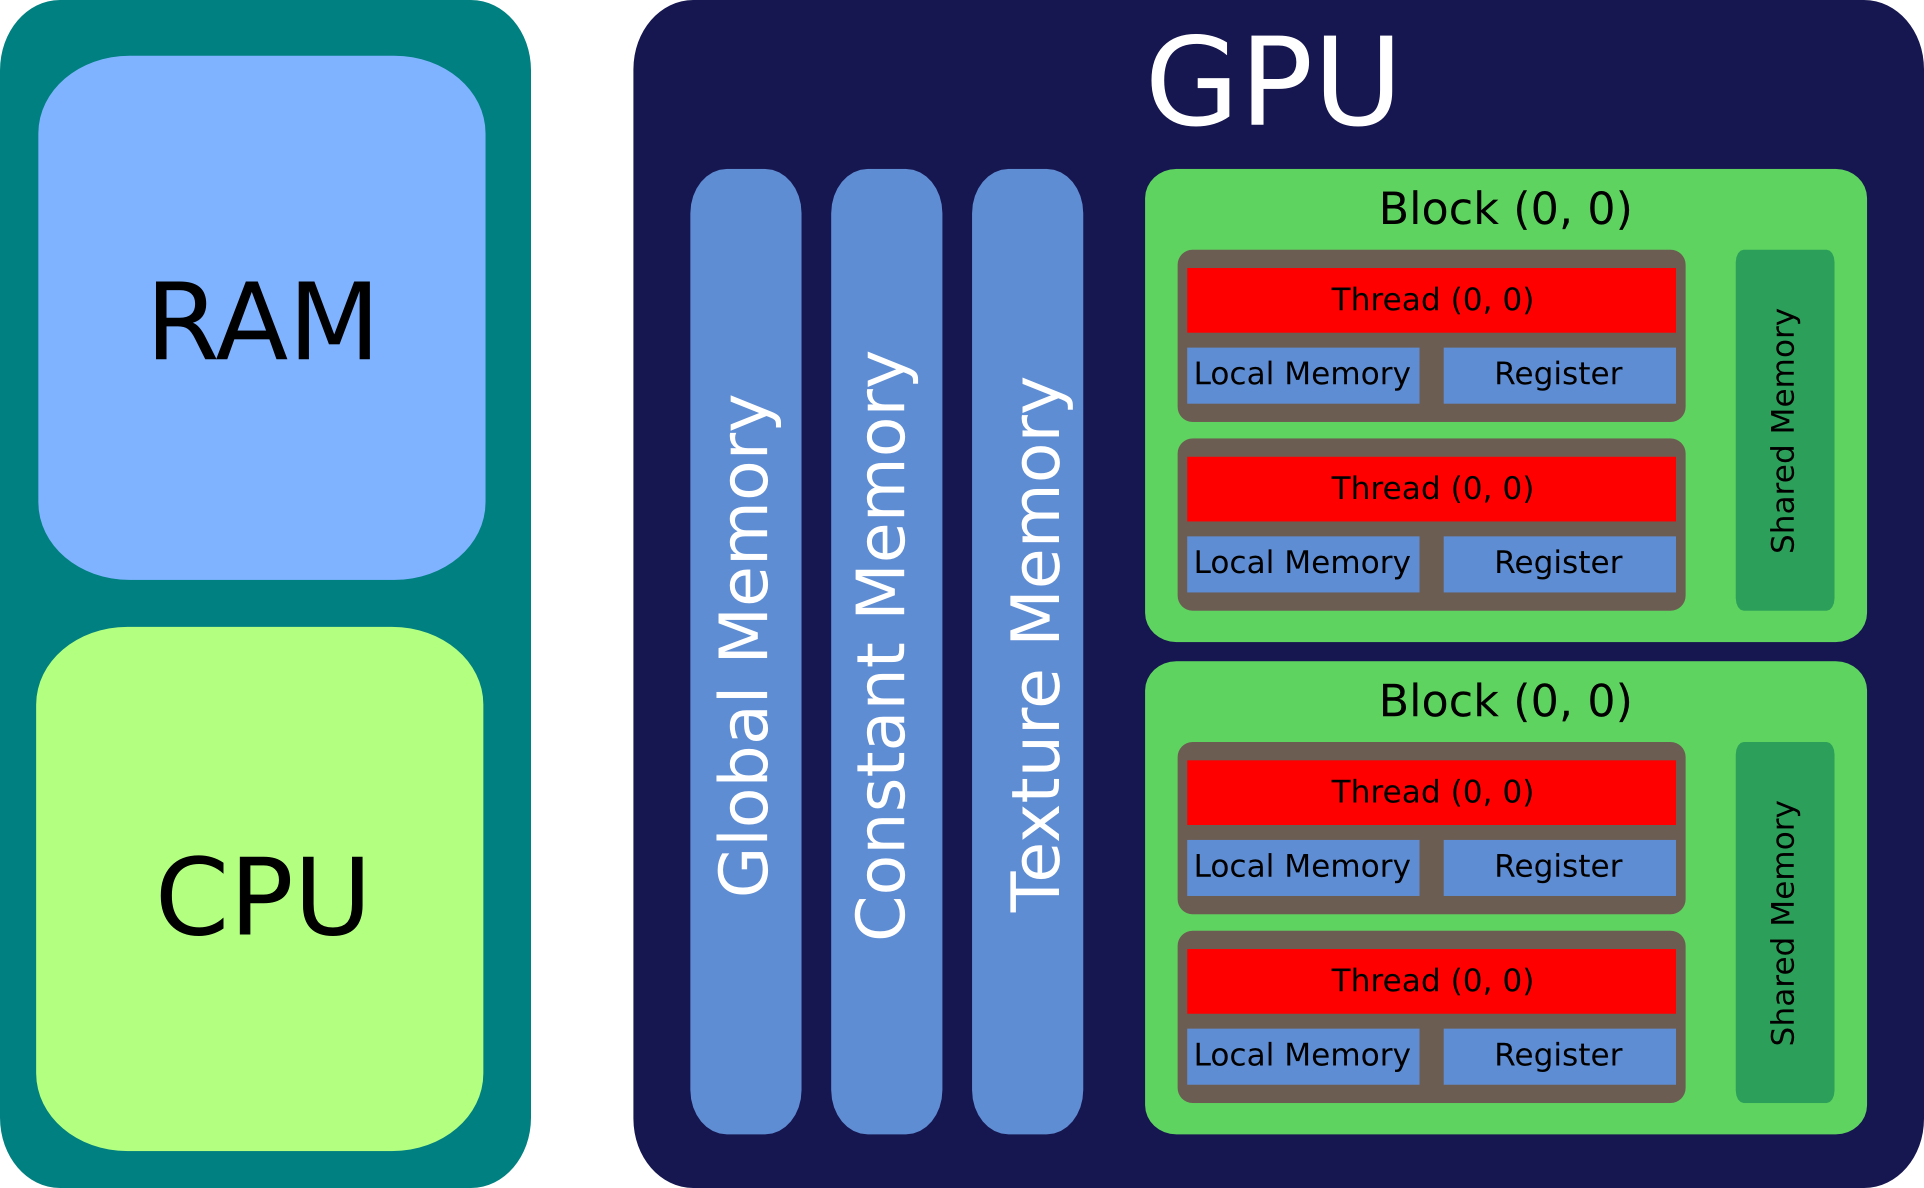
\includegraphics[width=0.8\textwidth]{gfx/cuda/gpu.png}\label{fig:gpu_arch}
  \caption{Speicherlayout einer Nvidia-GPU}
\end{figure}

-bild
-speicher bereiche
-grid layout function call
-threadidx etc

\section{Algorithmus}
-oder so ?
-erläuterung  implementierung
-speicherverwaltung

\section{Optimierung}
- coalesceded
- bank conflicts?
- teilvolumen nicht rechnen

\section{Validierung}
- beispiel rayleigh benard system
- masa
- vgl o2 vs o4 masa cube
- bifurcation


\newpage


\chapter{Python Simulation API}

\section{Introduction}

In this chapter we want to give a brief overview to the high object oriented simulation API which
was written in the context of this thesis, with the python programming language.
The purpose of the library in general is to simplify the execution of simulations, but furthermore
includes the possibility to analyse the results and use visualization techniques to study the overall
behaviour of the simulations during runtime.
Before we talk about the general workflow with the API, we first want to introduce the usage
and concepts of the different API classes and objects.

\section{Parameter File}

The Parameter File contains every flag and parameter which is used during the runtime of the simulation.
During compile time all parameters are converted into a specific set of C-macros which are then compiled
into the cuda code. As a file format we choose the open-standard format \textbf{Json} \footnote{Javascript Object Notation},
which is human-readable and furthermore very easy to parse in any programming language.
An example of a Parameter file is shown in Listing ()
The parameter file contains of two sections.
\begin{enumerate}
\item{conditions} Flags which are set to a constant value during runtime mostly zero or one. For example the boundary conditions and
                  interpolation methods. Not all flags have to be set for a simultaion.
\item{parameters} The parameter set defines all parameters which care used  for a simulation. In contrast to the conditions, each
                  parameter has to be defined in order to enable a proper execution.
\end{enumerate}
\begin{minipage}{\linewidth}
\begin{lstlisting}[language=json,firstnumber=1, caption='Example of a "paramater.json" file.]
{
    "conditions": {
        "all_periodic" :1
    },
    "parameters": {
        "BLOCKSIZE": 8,
        "STEPMAX": 200000,
        "IC_NAME": "\"c2_1000\"",
        "RAYLEIGH":0,
        "DELTA_T": 0.0001,
        "SOUND_SPEED_SQUARED": 400,
        "PRANDTL": 0.01,
        "GPU_ID": 2,
        "EKMAN": 0.0001,
        "NX": 64,
        "NY": 64,
        "NZ": 8,
        "LX": 1.0,
        "LY": 1.0,
        "LZ": 0.125,
        "RUN_NAME": "\"c2_1000\"",
        "NUM_GPU": 1,
        "SAMPLING_RATE": 5000,
        "NX_D": "NX/NUM_GPU",
        "NU": 0.0001,
        "PM": 1,
        "KAPPA": 0.0001
    }
}
\end{lstlisting}
\end{minipage}

\section{Generator Class}

The generator class is responsible for the generation of all initial data.
This means the initial conditions for all variables i.e. velocity and temperature
and the computation of interpolation and domain masks which are necessary for the different
immersed boundary methods.\\
During the execution of a simulation all precomputed arrays are stored within a
HDF5-File format, which is optimized for the storage and structuring of large amounts of data.
Furthermore the format simplifies the data exchange between the python api and the cuda programm.\\
For the generation of data a generator object has to be initialized with a generator function,
there are currently implemented three types of these functions.

\begin{description}
\item[Initial  Conditions] These functions simply generate the initial conditions for a certain flow problem, for example the taylor couette
                            flow or a simple cylndric domain. The definition of the functions can be found in pycurb.ic
\item[Testcase] The testcase functions extend the initial conditions by having the possibility to add certain forcing parameters into the timestep
                for example a pressure gradient is necessary for the poiseuill-flow setup described in section ().
                All defined functions can be found in pycurb.testcase.
\item[MASA]     MASA functions enable the possibility to perform a  manufactured solution analysis, by defining a solution of the flow problem.
                The python api then computes additional source terms from the navier stokes equation which are inserted into the equations of motion (see section ()).
                All defined functions can be found in pycurb.mase
\end{description}


It should be noted that it is quit easy to add a new function to the library, an example for an ic function definition can be found in appendix (x).
Additionally it is possible to create a generator which takes the data from an old simulation. In listing () the creation of a generator object is
exemplary shown. At first the generator is created by using a generator function, afterwards it is possible to define certain attributes
for example the radius of a cylindric fluid domain.\\

\begin{python} [caption='Generator class usage']
import pycurb as pc #import the simulation API
import pycurb.testcase as tf #import testcases
import pycurb.ic as as ic    #import initial conditions

#create a generator object for pipe flow in z direction
generator = pc.Generator.from_testcase(tf.cylinder_flow_z)
#set the default velocity profile, pressure gradient and radius
generator.add_option('SETV', True)
generator.add_option('PMAX', pmax)
generator.add_option('r', 1.)

#create a generator object for taylor couette flow
generator = pc.Generator.from_ic(ic.taylor_couette)
#set velocity, inner and outer radius
generator.add_option('SETV', True)
generator.add_option('ri', ri)
generator.add_option('ro', ro)
\end{python}

\section{Simulation Class}

An intance of the simulation class is the main object of the API and
necessary to execute a simulation. For the creation of a simulation object
the initial arguments are the filepath where all simulation data will be stored
and the json-file for the parameter setting.
Following the creation of the simulation object it is possible to alter all parameters and conditions
which were previously stored in the json-file. This gives the possibilty to create
simulations with different parameter settings on the fly, i.e. change the resolution of the numerical grid
to perform a grid convergence study.
Before the execution of the cuda code, the simulation object has to be bind to a generator object
with the \textbf{generate\_files} class function, in return the generator object will begin
with the data creation. The last step is execution of the cuda code which can be done with the \textbf{start\_simulation}
class function.  A minimal usecase of the complete procedure shown in listing (X).


\begin{python}[caption='Generator class usage']
import pycurb as pc
import pycurb.ic as ic

generator = pc.Generator.from_ic(ic.taylor_couette)
sim = pc.Simulation('data', 'parameter.json')
sim.parameter.set('NX', 128)
sim.parameter.set('NY', 128)
sim.parameter.set_condition('o2', order)
sim.generate_files(generator)
sim.start_simulation()
\end{python}

\section{Usage Example}

Finally we want to give a usage example for a grid convergence study using
the Simulation API. The source code is shown in listing (X).
In the example we simulate a pipe flow, for a more detailed discussion we refer to section ().
We start by importing the relevant modules from the API and defining all relevant constants like the
Reynolds number, $Re=100$ in this case.
Finally we create and loop over an numpy array which contains all resolutions on which we want to test
our fluid problem.\\
Inside the for loop we begin by defining a unique simulation path for each resolution.
The we create the generator with the pipe-flow settings from the \textbf{pycurb.testcase} module and
the options for the pressure gradient, the initial velocity field and the pipe radius.\\
Finally the simulation object is created, here we set all parameters like resolution and domain size,
the order of the finite difference scheme and the direct forcing method which will be introduced in section ().
The last step is to execute a single simulation.\\
The given example is build to be executed on a single machine in order to further parallize the computations on
more than one gpu an additional python script \textbf{worker.py} was written which is not yet included in the simulation API (see Appendix A(XX)).
To parallelize the example some small adaptions has to be made. For each resolution the simulation path has to be stored into a textfile, which
is than opened by the python script, furthermore the execution of the simulation has to be removed from the for-loop.
Finally we start by generating all simulation data by executing the modified version of our script. Afterwards we start
the parallelization script for which we have to specify the file including the simulation path and the number of gpus and cuda machines we want to use.

\begin{python}[caption='Grid Convergence Study Example']
import pycurb as pc
import pycurb.testcase as tf
import numpy as np
import os

def main():
    #define simulation parameters
    re = 100.
    pmax, pr = 4./re,  1./re
    lx, ly, order = 2.5, 2.5, 1

    #vary N from 16 to 256 with dN=16
    res = np.linspace(16, 256., 256./16)

    for rs in res:#iterate through resolution array
        #create filepath for each simulation
        var_path = os.path.join(method,'res_%i' % rs)
        sim_path = os.path.join(os.path.dirname(__file__), "data", var_path)

        #create generator with simulation settings
        generator = pc.Generator.from_testcase(tf.cylinder_flow_z)
        generator.add_option('SETV', True)
        generator.add_option('PMAX', pmax)
        generator.add_option('r', 1.)

        #create simulation object and set parameters
        sim = pc.Simulation(sim_path, "parameter.json")
        sim.parameter.set("PRANDTL", pr)
        lz = dx*(lx/rs)
        sim.parameter.set("NX", rs)
        sim.parameter.set("NY", rs)
        sim.parameter.set("LX", lx)
        sim.parameter.set("LY", ly)
        sim.parameter.set("NZ", nz)
        sim.parameter.set("LZ", lz)
        sim.parameter.set_condition('o2', order)
        sim.parameter.set_condition('SET_ZERO', 1)
        sim.generate_files(generator)

        #execute simulation
        sim.start_simulation()

if __name__=='__main__':
    main()
\end{python}

The script creates a thread-safe queue and a number of threads, one for each gpu per machine.
Each thread automatically fetches a job from the queue, than logs into the assigned cuda machine
and executes the job on the given gpu.
For time consuming simulations also a modificated version of the script was written where one thread
can use more than one gpu, see Appendix A(XX).


\chapter{Immersed Boundary Methods for No-Slip Walls}
\section{Overview of Immersed Boundary Methods}

\begin{figure}[!bp]
  \centering
  \subfloat[cartesian grid]{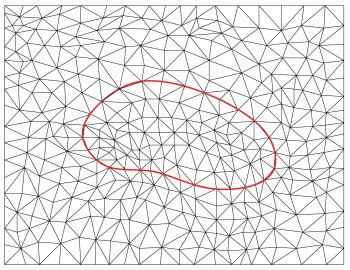
\includegraphics[width=0.4\textwidth]{gfx/immersed_boundary/general_partition_triangle.jpg}\label{fig:grid_f0}}
  \hfil
  \subfloat[unstructured body-fitted grid]{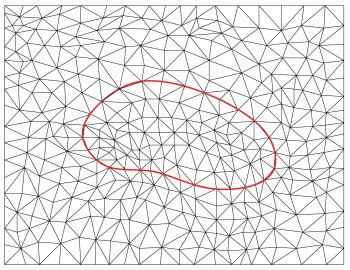
\includegraphics[width=0.4\textwidth]{gfx/immersed_boundary/general_partition_triangle.jpg}\label{fig:grid_f2}}
  \caption{Different types of numerical grids}
\end{figure}

For many fluid problems it is mandatory to solve the equations of motion with respect to complex-shaped geometries \.
The algorithm introduced in section () is not yet suitable for such a scenario.
For instance the simulation inside a spheric geometry is impossible, since the boundaries
do not coincide with the implemented cartesian grid. Nevertheless there exist different approaches to overcome this problem,
which shall be introduced here. \\
The common approach to extend the algorithm would be to use a body-fitted mesh (see figure \ref{fig:grid_f1}),
different advantages and disadvantages arise with this kind of implementation (see \citep{Mittal2005}).
One benefit is a much simpler deployment of the desired boundary condition, due to the overlap of the grid with domain border.
Furthermore a higher accuracy can be achieved \citep{Gornak2013}.
However, using an unstructered grid generates plenty of computational overhead, during and before the execution of a simulation.
The generation of the grid is very complicated in contrast to using a cartesian grid, this can be even more complicated when
considering moving boundaries.
Also solving the finite differenc schemes on a curvilinear coordinate system, leads to more calculations on a single grid point.
The last important aspect is the implementation on the gpu.
Like discussed in section () it is more efficient to use homogenous storage and calculation pattern on a CUDA-device,
the use of unstructured data makes this very difficult.
Altough some attempts exists to solve these difficulties (see i.e. PAP), it is still uncertain if the obtained performance loss would be acceptable.\\
A set of alternative methods, to resolve the problems described above, are so called Immersed Boundary Methods.
The term was first mentioned in (PESKIN 1972), for the simulation of blood flow through a heartvale, but has since then been used for a variety of
methods (MITTAL).  All of them have the idea in common to perform the simulations on a cartesian grid which does not conform to the domain boundary.
To satisfy the desired boundary conditions additional terms are introduced into the equations of motion.
In general one can distinguish between contiuous forcing methods and direct forcing methods.
Continious forcing methods try to mimic the boundary using a localized force which acts on the boundary,
since the surface is tracked by lagrangian points this methods can be well suited for moving boundaries (MITTAL).
One common problem is that continous forcing can arise to stability problem and numerical oscillations in numericial stiff problem (SOURCE).
The direct forcing approach tries to satisfies the boundary condition, by imposing it directly to points near the fluid surface for example
trough an interpolaltion procedure.
Some of the major drawbacks using the IBM is the loss in  spatial accuracy at the boundary, therefore it can be necessary to use a higher grid resolution
compared to a body-fitted mesh.  Futhermore the non-conforming (?) boundaries are more difficult implement.
The benefits of these methods is the use of a cartesian grid, which is much more suited for a gpu-based implementation (see section X).
As a result the overall performance will probably be in the same order as the original algorithm.
In the thesis the Implementation of different Immersed Boundary Methods is seperated into three chapters depending on the boundary condition and application.
This chapter beginns with Implementation of NoSlip-Walls which are the easisest to implement.
The term Immersed Boundary Method is vaguely defined in literature, in this thesis we refer to it with all methods introduced in the following three chapters.


\newpage

\section{Implemented Methods}

For the purpose of discussion, the different methods introduced here, will be applied to a default geometry.
The fluid domain without any immersed boundaries is set to a cube of the size $l_i= 1$ with  $i = \{x, y, z\}$.
For the discretization we choose $N_i = 32$ for the number of grid points.
As an example of an immersed boundary, we will dicuss the embedding of a cylinder, given by the  surface equation

\begin{align}
    \left(x - \frac{l_x}{2}\right)^2 + \left(y - \frac{l_y}{2}\right)^2 = r^2
\end{align}

where $r=0.4$ is the radius and the center is given by $(l_x/2, l_y/2)$. The whole setup is schematically shown in figure (X).
The simulation domain is than seperated into the fluid domain $\Omega_f$ and the wall domain $\Omega_w$.
The overall goal is to enforce the no-slip condition $\vec{v} = 0$ on the surface $\partial \Omega_f$, furthermore
the consveration of mass should be fulfilled.

\subsection{Volume Penalization}

\begin{figure}[!b]
    \subfloat[Cylinder geometry of the immersed boundary embedd in the simulation domain]{{
      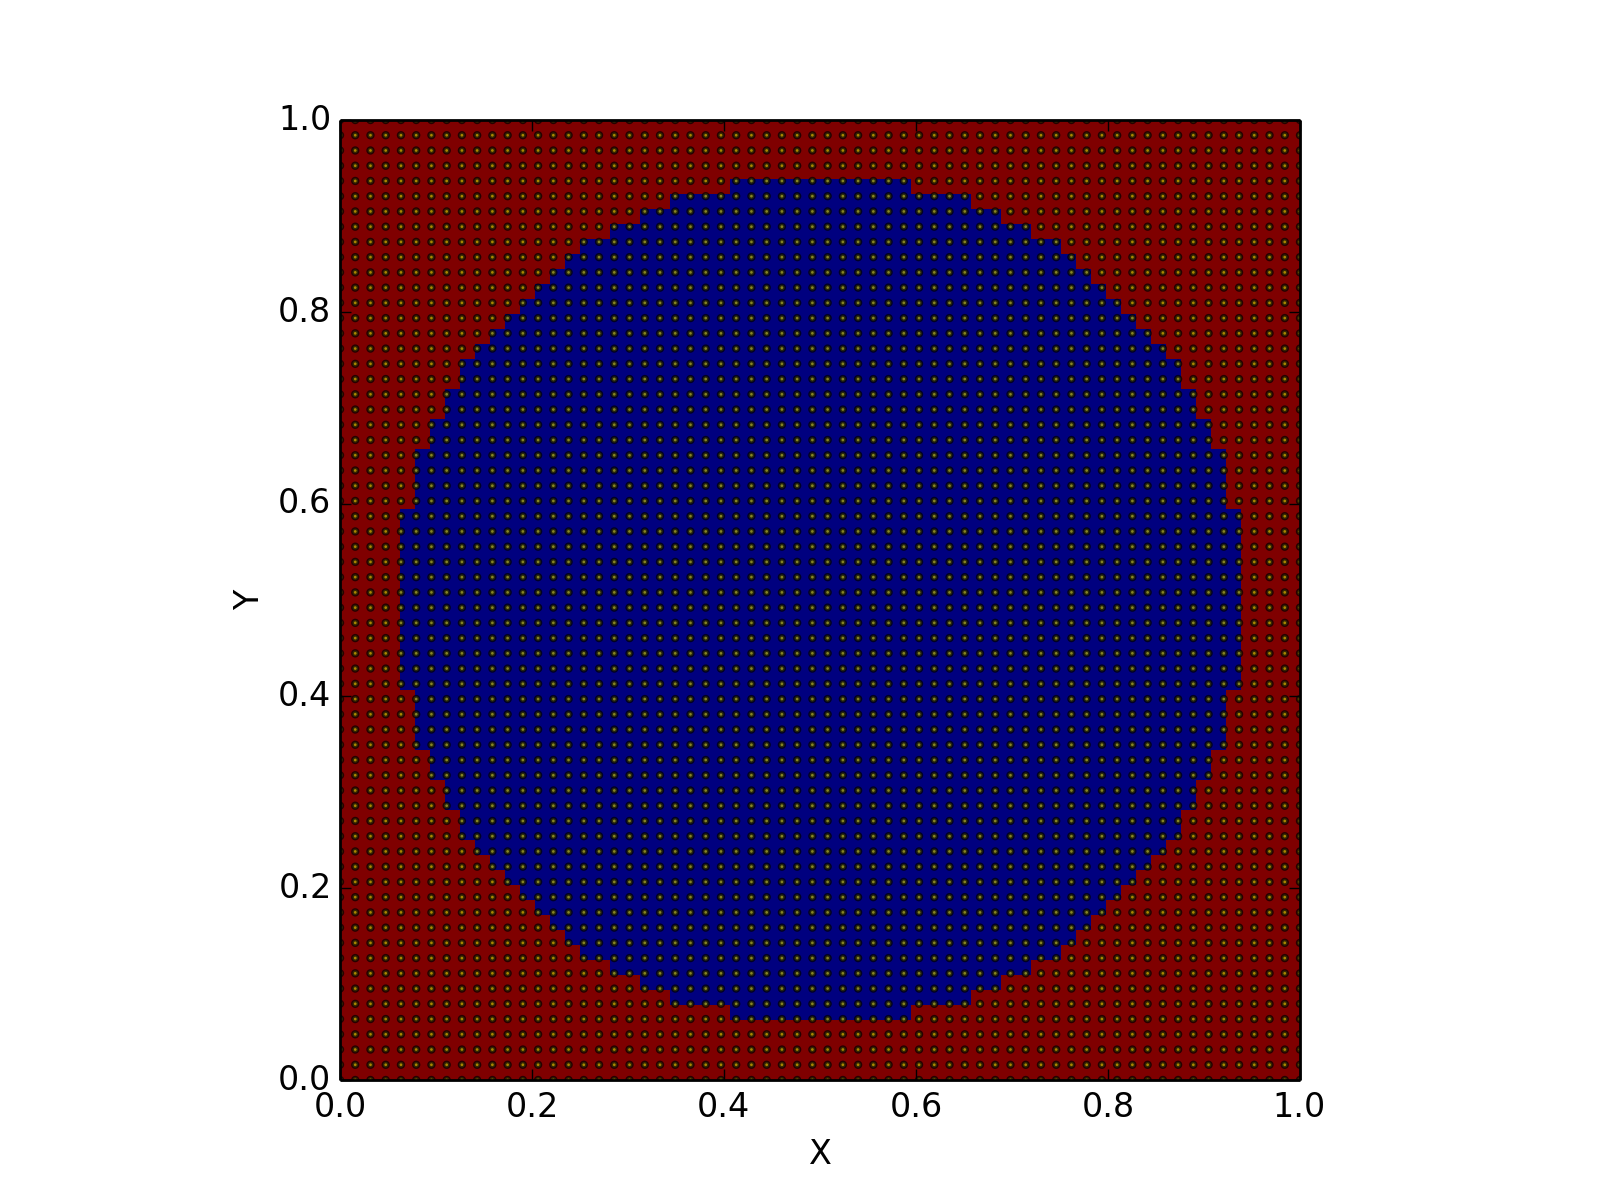
\includegraphics[width=0.5\textwidth]{gfx/immersed_boundary/mask.png}\label{fig:mask_vp}
        }}%
    \subfloat[Masking function $H(x,y,z=const.) = x^2 + y^2 < c$ for a cylinder. ]{{
      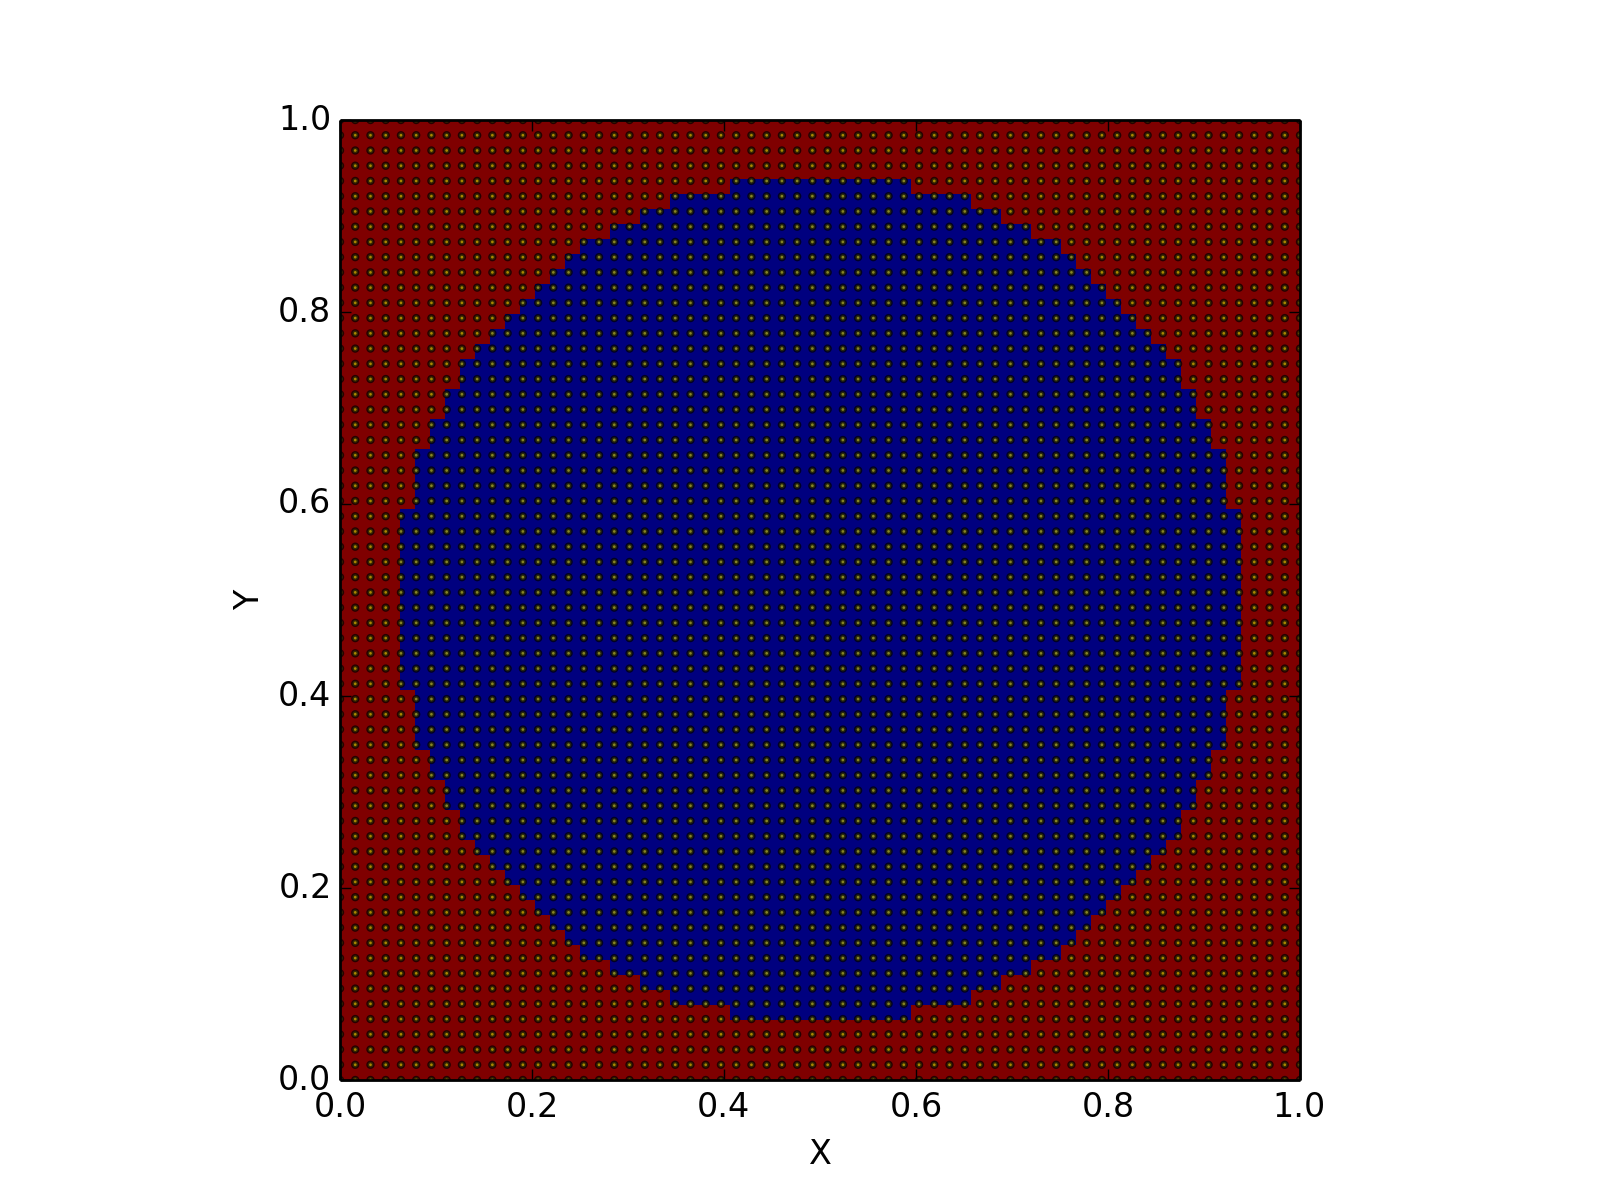
\includegraphics[width=0.5\textwidth]{gfx/immersed_boundary/mask.png}\label{fig:mask_vp}
     }}%
    \label{fig:example}%
\end{figure}

The idea behind the volume penalization method is to introduce an additional forcing term into the Navier-Stokes equation, which acts on
the grid points outside of the fluid domain to ensure the desired boundary conditions. The methods was sucessfully implemented and tested
on pseudo-spectral methods, see for example (CITE).
For the implementation it is necessary to define a masking function $H(x, y, z)$ which seperates the simulation domain into $\Omega_f$ and $\Omega_w$.
In case of the cylinder, we can use the surface equation (REF) and simply obtain.
\begin{align}
H(x, y, z) = \begin{cases}
                    0, &  \left(x - \frac{l_x}{2}\right)^2 + \left(y - \frac{l_y}{2}\right)^2 <r^2\\
                    1, & \text{else}
             \end{cases}
\end{align}
Now we can introduce an additional forcing term into the impulse equation,
\begin{align}
    \pdn[u]{t} + \vec{u} \cdot \vec{\nabla} \vec{u} &= -c^2 \nabla \rho + \frac{1}{Re} \Delta \vec{u} + \vec{F}_{ext}
     +\underbrace{ \frac{H(x, y, z)}{\nu}(\vec{v} - \vec{v_0})}_{\text{damping force}}
\end{align}

where $\vec{v}_0$ conforms the desired boundary condition, i.e. $\vec{v}_0 = 0 $ for no slip boundaries, and $\nu$ is a regulation parameter also denoted as damping rate of the forcing.
The additional term acts as an exponential damping force on a single gridpoint inside of $\Omega_w$, by the product with since it vanishes in $\Omega_f$ by the definition of $H(x,y,z)$.


Die Antwort des Kraftterms wird durch die Dämpfungrate $\nu$ reguliert. Je kleiner $\nu$ desto stärker ist die Dämpfungsrate, allerdings kann der Term
nicht beliebig klein gesetzt werden da die Stabilität für $\nu < dt$ nicht mehr gewährleistet ist [source].
Da für die Lösung der der Geschwindingskeitsfelder mit der Methode der künstliche Kompressibilität  bereits ein sehr kleiner Zeitschritt verwendet wird (s.Abb. X)
kann im Vergleich zu anderen Verfahren wie z.B. (pseudo-spektrale) eine relativ starke Dämpfungsrate verwendet werden.
-konvergenz nu gegen 0 MPI\\
- stiff probplem dt < dtpen = nu DIPLOM\\
- dary type law MPI\\
\newpage


\subsection{Direct Forcing}
Während die Volume Penalization Methode die Geschwindigkeit ausserhalb des Volumens nicht vollständig auf Null setzt,
 kann dies durch eine implizite Berechnung des Dämpfungsterm erreichtwerden. Es stellt sich heraus das dieser Ansatz equivalent
  zu der Direct Forcing Methode ist, die erstmals von [] verwendet und in [] beschrieben wird.
Betrachten wir zunächst den diskretisierten Zeitschritt
\begin{align}
    \frac{\vec{u}^{n+1} -\vec{u}^n}{\Delta t} = \mathscr{L} + \vec{f}\\
\end{align}
wobei $\mathscr{L}$ den diskretiesierten Operatoren der PDE entspricht.
Für einen Punkt auf dem Rand des Volumens soll nun die Randbedingung $\vec{u}^{n+1} = \vec{u}_0$ eingehalten werden.
Mit Formel () folgt
\begin{align}
    \frac{\vec{u}_0 -\vec{u}^n}{\Delta t} = \mathscr{L} + \vec{f} \Rightarrow \vec{f} = \frac{\vec{u}_0 -\vec{u}^n}{\Delta t\cdot \mathscr{L}}\\
\end{align}

Mit der Annahme dass der Rand mit dem numerischen Gitter übereinstimmt ist es nicht nötig den Kraftterm zur berechnen, stattdessen lässt sich der
Schritt vereinfachen in dem der Randwert nach  jedem Zeitschritt direkt auf die gewünschte Randbedingung gesetzt wird. Durch die
implizite Behandlung kommt es zu keiner weiter Stabilitätsbedingung.

\newpage

\subsection{Volume Fraction Interpolation}

The methods introduced up to here lack the ability of an exact impementation of the boundary conditions on $\Omega_f$.
Instead the surface $\partial \Omega_f$ is described by the nearest grid points in $\Omega_w$, resulting in an
stepwise approximation.
To overcome this problem a simple procedure is the use of an volume fraction interpolation scheme, introduced in [FADL].\\
The advantage of this method is the simple implementation into the volume penalization and direct forcing method.
Furthermore the overall computation time of the timestep stays constant, in  contrast to complex interpolation schemes.\\
Initially the interpolation beginns by determine all grid cells\footnote{definition cell} which are cut by the surface $\partial \Omega_f$.
For each of these boundary cells the total volume $V_w$ of the wall domain $\Omega_w$, inside each cell, is computed.
The force acting on the points inside the boundary cells is than weighted by a scaling factor, $\Phi = V_W/(\Delta x \Delta y \Delta z)$.
For the volume penalization method the scaling is simply multplied with the forcing term in eq. ().
Since the implementation of the direct forcing method is setting the velocity components directly to zero, it is necessary to
fall back to equation () and introduce a forcing term

\begin{align}
    \vec{f} = \Phi \frac{\vec{u}_0 -\vec{u}^n}{\Delta t\cdot \mathscr{L}}\\
\end{align}

\begin{figure}[!bp]
    \centering
    \subfloat[label 1]{{
      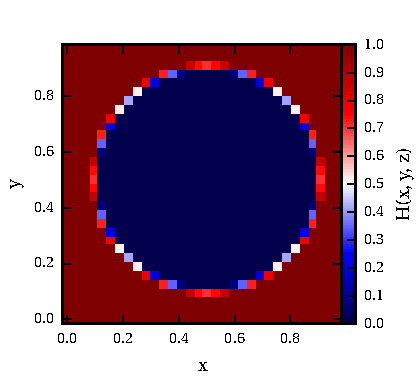
\includegraphics{gfx/immersed_boundary/methods/mask_volfrac.pdf}\label{fig:mask_volfrac}
        }}%
    \qquad
    \subfloat[label 2]{{
      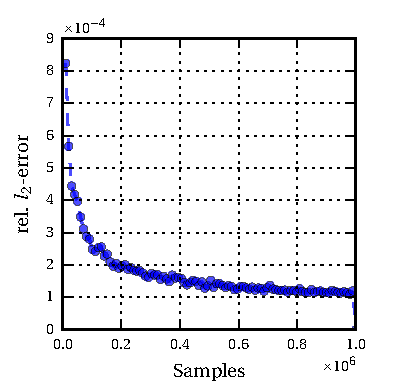
\includegraphics{gfx/immersed_boundary/methods/error_volfrac.pdf}\label{fig:error_volfrac}
        }}%
    \label{fig:example}%
\end{figure}

Since the operator $\mathscr{L}$ is computed during the first part of the time step. This forcing term can added during the completion of the runge kutta step.\footnote{see section}\\
For the implementation of an extended version of the masking array $H$ is used.
Like in the previous methods the masking array is precomputed and loaded at runtime. The algorithm is extended to compute the
volume fractions of the cells lying next to the surface $\partial\Omega_f$.
Since an exact computation is difficult to implement for abritary surfaces, the idea is to use a monte carlo integration method.
For each cell $N$ random samples are generated, then the volume fraction is simply given by the ratio of samples lying in- and outside ot the domain.
The implementation into a simulation class using the python API is explained in more detail in Appendix ().\\
An example for the computed masking array with $N=2e5$, is shown in figure (). The symmetric distribution of the boundarie values indicates
a good approximation, for a better evaluation a convergence study was performed were the number of samples $S$ was varied between 100 and $10^6$ points.
The $l_2$-error was determined by comparing the results to the computation with the highest number of samples.
The results are shown in figure ().\\

-discussion for n>10000 error 1e-5\\
-overall good approximation \\
-erweiterung  *2 etc blabla\\



\subsection{Interpolation}
\newpage

\section{Validation}

In order to ensure a correct numerical behaviour of the introduced methods,
a large part of the thesis deals with the numerical validation.
Multiple examples from simple to more complex testcases are introduced in this section.
In general it is necessary to obtain a good evaluation of the numerical truncation error, the numerical stability over longer periods of time
and the fullfilment of the conversation laws, most importantly mass conservation.
Grid convergence studys against theoretical and high-resolution numerical solutions  will be performed
and compared for the different IBMs.


\subsection{Laminar Poiseuille-Flow}
\subsubsection{Theoretical description}

\begin{figure}[!bp]
  \centering
  \includegraphics[width=0.8\textwidth]{gfx/immersed_boundary/val_volpen/poiseuilleflow.png}\label{b}
  \caption{Theoretical setup of the poiseuille-flow channel.}
\end{figure}

%\begin{wrapfigure}{r}{0.5\textwidth}
%  \begin{center}
%      \includegraphics[width=0.48\textwidth]{gfx/immersed_boundary_methods/val_volpen/poiseuilleflow.png}
%   \end{center}
%          \caption{ paxvleb xvle}
%\end{wrapfigure}


The first testcases is the laminar poiseuille-flow, the theoretical setup is presented in figure ().
It consist of two infintiy long planes at $z=h_1$ and $z=h_2$, which are oriented parallel to the xy-plane and the distance $\Delta h = h_2 - h_1$ between them.
Numerically this is realized by using periodic boundaries in xy-direction and no-slip boundaries in z-direction.
The velocity profile results from an external force, given by a  pressure gradient in x-direction, which is introduced into the naviers-stokes equation.
No other forces are present furthermore the flow will be independent of the y coordinate,
hence for the steady state $\partial v_x /\partial t = 0$ the equations of motion can be reduced to:

\begin{align}
\frac{\partial v}{\partial t} &= - \frac{\partial p}{\partial x} + \nu \frac{\partial^2 v_x}{\partial z^2} = 0
\end{align}

where v is the velocity in x direction.
For the non-dimenzionalization we choose $r^* = r/L$, $v^*=v/L$, $t^* = \frac{V}{L}$ and $p^* = p \rho V^2$ where $L=\Delta h$ and $V=v_{max}$.
The non-dimensional equation reads

\begin{align}
\frac{\partial v}{\partial t} &= - \frac{\partial p}{\partial x} + \frac{1}{Re} \frac{\partial^2 v_x}{\partial z^2} = 0
\end{align}

with $Re = VL/\nu$.
For the volume penalization method we furthermore obtain a non-dimensional damping force $-\frac{H}{J}\cdot v$ with $J = VL/\eta$.
The equation can simply be integrated twice which yields the solution

\begin{align}
v &= \frac{1}{2}\frac{\partial p}{\partial x}z^2 + zc_1 + c_2
\end{align}

Using the noslip-boundary condition $v_x(h_1) = v_x(h_2) = 0$ and furthermore by defining
$A:=\frac{1}{2}\frac{\partial p}{\partial x} Re$ one obtains the additional conditions

\begin{align}
c_1 &= A\frac{h_1^2 -h_2^2}{h_2 - h_1} = -A(h_1+h_2)\\
c_2 &= A(h_1(h_1 + h_2) - h_1^2) = Ah_1h_2\\
\end{align}

The velocity is than given by the quadratic function

\begin{align}
v_x &= A(z^2 - z(h_1 + h_2) + h_1h_2)
\end{align}

The maximum velocity and postinon can be obtained by simple calculus

\begin{align}
z_{max} &= \frac{h_1+h_2}{2} \wedge v_{max} = A\left(h_1h_2 - \frac{(h_1 + h_2)^2}{4}\right)
\end{align}

Since $v_{max}$ has to be 1 by definition of the non-dimensionalzation we find

\begin{align}
\frac{\partial p}{\partial x} &= \frac{2}{Re}\frac{1}{\left(h_1h_2 - \frac{(h_1+h_2)^2}{4} \right)}
\end{align}

as a necessary condition for the pressure gradient.\\
With the given theoretical solution, the next objective is the comparison
to the default implementation, the volume penalization method and the direct forcing method.
Since we have a flow parallel to the grid  it does not make sence to compare it to the interpolation methods
For the comparision with a theoretical solution it is necessary to ensure that the surface grid points match with the total height $h$ of the channel.
In the default setup tes gibthe noslip-boundaries are realized with the default implementation, like explained in section ().
For the immersed boundary methdos the upper- and lower boundaries are given by the masking function.
\begin{align}
H(x, y, z) = \begin{cases}
                    0, & \text{for \  }  z < h_2 \lor z>h_1 \\
                    1, & \text{else}.
             \end{cases}
\end{align}

\subsubsection{Test of the Default Implementation}

\begin{figure}[!bp]
    \centering
    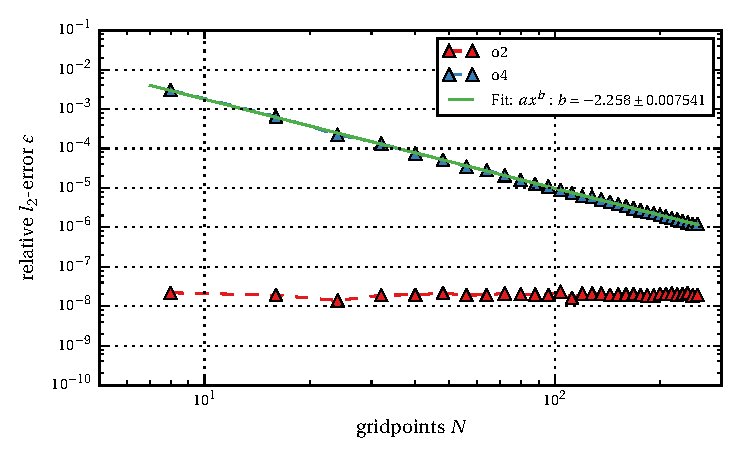
\includegraphics{gfx/immersed_boundary/poiseuille_flow/1_default/relative_l2error.pdf}
    \caption{Relative $l_2$-error for second and fourth order schemes of the default algorithm.\label{fig:ema1}}
\end{figure}

Initially a grid convergence test was performed with the default implementation of the algorithm, without the use of immersed boundaries.
For this test case this is still possible since the geometry is non-curved and parallel to the cartesian grid.\\
For the  numerical setup the parameters were set to $l_x=1$, $l_y=0.25$, $l_z=1$.
The reynolds number was set to a constant value of $Re=500$, whereas the resolution $N$ was varied in the Intervall $[16 - 128]$ with a stepsize of $\Delta N = 8$.
The timestep was set to $\mathrm{dt}=1e-5$ and the pressure gradient to $\partial p \partial x  = 10$.
For all resolutions the simulations were performed for finite differcen schemes of second and fourth order.
The results are shown in figure \ref{fig:ema1} on a double logarithmic plot.\\
For the finite difference scheme of second order, the error behaves not as assumed.
Instead of the decline one would expect with the decrease of the resolution, the  error is nearly constant.
This behaviour can be explained due to the lack of complexity of the test case. As the theoretical solution is a polynom of second order
no higher order terms will occur in the numerical solution, hence the second order scheme is capable of a perfect approximation, independent of the
grid resolution. The remaining error terms, are of the order $10e^{-8}$, which is extremly small and occur due to the floating point round off.
With this in mind the behavior of the fourth-order scheme is even more unexpected.
We see a linear decrease of the error on the log scale.
The result of a power law fit yields a convergence rate of second order.
Furthermore the error is much larger compared to the second order scheme, there is a decrease from $10e^{-2}$ to $10e^{-5}$.
The test case reveals that an error exists in the default implementation of the boundarie conditions.
An explanation can be given with comparison of the theoretical solution. The laplace operator is given by
 $ \nu \pdn[^2 v_x]{x^2} = 2A = \frac{1}{\nu}\pdn[p]{x}$
Using the mirroring method creates a discontinuous function at the boundaries, since the laplace operator changes the sign.
When using the second order method the tree-point-stencil evaluates to the correct value $\pdn[^2 v_x]{x^2} = 1$.
The five-point-stencil of the fourth orderer scheme evaluates to $\pdn[^2 v_x]{x^2} = 1$, since it uses one point behind the boundary.
As a result the discontinuity creates an error in the higher order scheme.\\
For this testcase the second order method yields better results, however we
have to keep in mind that the testcase yields a polynomial solution,
it is not clear how the results will end up for a complex testcase.
Furthermore in this testcase the boundaries have a large impact since the pressure gradient is parallel to wall,
his is not the case in general.
One possibility to avoid this error, would be to use an asymmetrich stencil, this approach is discussed in section ().

\begin{figure}[!b]
  \centering
  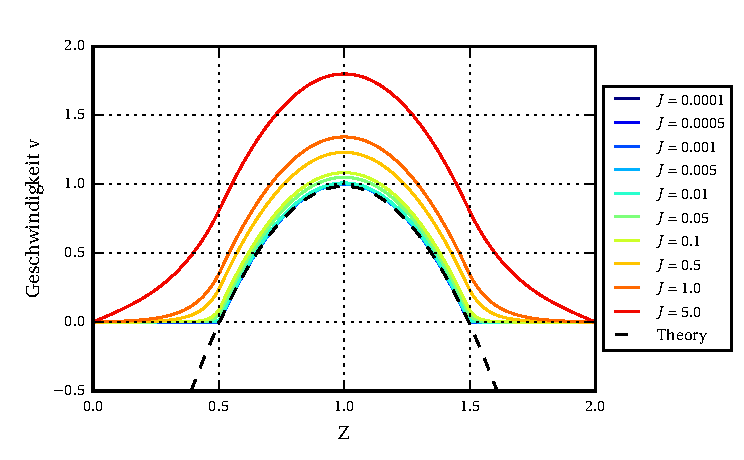
\includegraphics{gfx/immersed_boundary/poiseuille_flow/2_vp/vp_profile.pdf}\label{fig:vp_flow}
  \caption{Geschwindigkeistprofile im Kanal bei Variation der Dämpfungskonstante $\nu$ und Reynoldszahl $Re=500$.}
\end{figure}

\subsubsection{Test of the Volume Penalization Method}

The next objective is to investigate the error of the volume penalization method.
For this method the additional forcing term REFHERE is introduced into the equations. The non-dimenzionalzation leads to the form
\begin{align}
    \vec{f} = \frac{H}{J}v
\end{align}

with the quantity $J = 123$ as a non-dimensional forcing parameter.
(MACH NUBMER DISCUSSION HERE) \\
We begin by studying the behavior of the velocity profile, with variation of the Reynolds-number and the damping $J$, in the regime $Re=100-500$ and $\nu=1e-4 - 5e-1$.
The numerical setup is equal to the one for the default methods, except we now introduce the masking function (LABELABOVE) with $h_1=0.25$ and $h_2=0.75$.
To make sure that the channel width is equal to $\Delta h = 1$, the total height was set to $l_z\approx2.01587$. This furthermore ensures that the grid points overlap exactly
with the masking function at $h_1$ and $h_2$. The resolution was set to $N_x\times N_y\times N_z = 64\times16\times128$.
The resulting velocity profile is exemplarily shown in figure \ref{fig:vp_flow}, for varying $\nu$ and a constant reynolds number $Re=500$, for the second order scheme.\\
It can be noted that with an decrease of $\nu$, the numerical solution converges against the theoretical one.
The quadratic part of the velocity profile inside the fluid domain is independent of the damping constant $\nu$.
Since the damping can not fullfill the exact boundarie conditions, a slight offset is introduced into the velocity profile
which leads to an offset in the solution.
In the masked area of the volume we can see an exponential decrease of the total velocity.
Since for the steady state

\begin{align}
 \nu v &= D \frac{\partial^2 v_x}{\partial z^2}  \Rightarrow  v_x = A e^{\sqrt{\frac{\nu}{D}}v_x}
\end{align}

where A is given by the offset $v(h_1)$.\\
For an error estimation, the relative $l_2$-error was computed.
The results for the second order scheme are shown in figure \ref{fig:vp_error}.

\begin{figure}[!t]
  \centering
  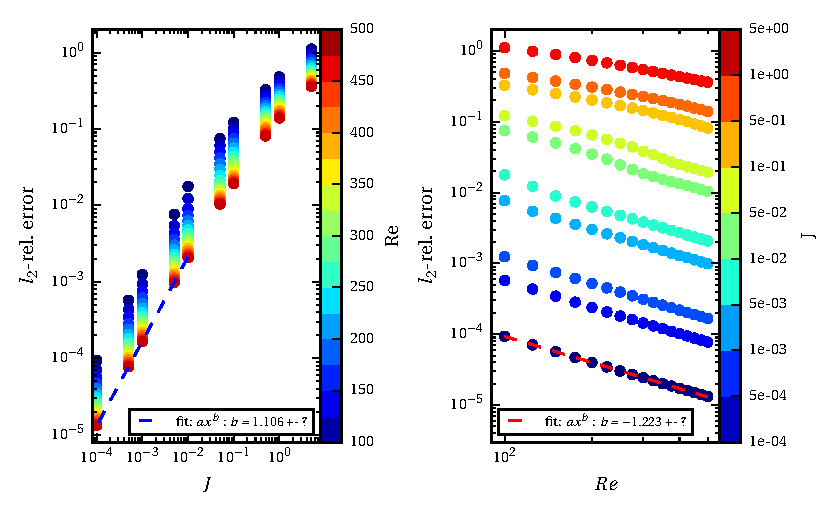
\includegraphics{gfx/immersed_boundary/poiseuille_flow/2_vp/vp_error.pdf}\label{fig:vp_error}
  \caption{Relative $l_2$-error for variable damping rate $\nu$ and reynolds-number $Re$.}
\end{figure}


The error decreases together with the damping rate from $1e-0$ to $1e-4$. For $nu<1e-3$ and a constant reynolds number we can observe an almost linear decrease in the logarithmic space,
this yiels a fit law of the form $ e = ax^b$. This shows that the error of this penalization method converges with first order in dependence of $\nu$.
The decrease for $nu>=1e-3$ can be explained by having a look at figure \ref{fig:vp_flow} again. Since the damping in the masking area is to
weak the flow sees the real boundaries of the fluid domains, which results in a stronger damping on the flow.
This is not the case for $nu<1e-3$ since the velocities reaches zero before reaching the boundarie.\\
Furthermore we can see a decrease of the error of one order with an increase in the reynolds number.
Since the damping force is proportional to the velocity and therefore to the reynolds number, the offset on the channel walls remains constant.
Due to the larger velocity profile this results in an smaller relative $l_2$-error, whereas the absolute error will increase.
For the fourth order scheme, the error is shown in figure APPENDIX.
We can observe a similar convergence  until the damping rate decreases to $\nu=1e-4$, below that value the error increases slightly to the order of magnitude of $1e-3$.
The reason for this behavior will be discussed soon.\\
Finally a grid convergence study was carried out, with a constant Reynolds number and $\nu \in [1-23]$.
The resolution was varied between $N\in [4, 400]$ with $\Delta N = 4$, second and fourth order schemes were tested.
For the correct solution the theoretical velocity profile (REF) was assumed.
The results are shown in figure().

\begin{figure}[!t]
  \centering
  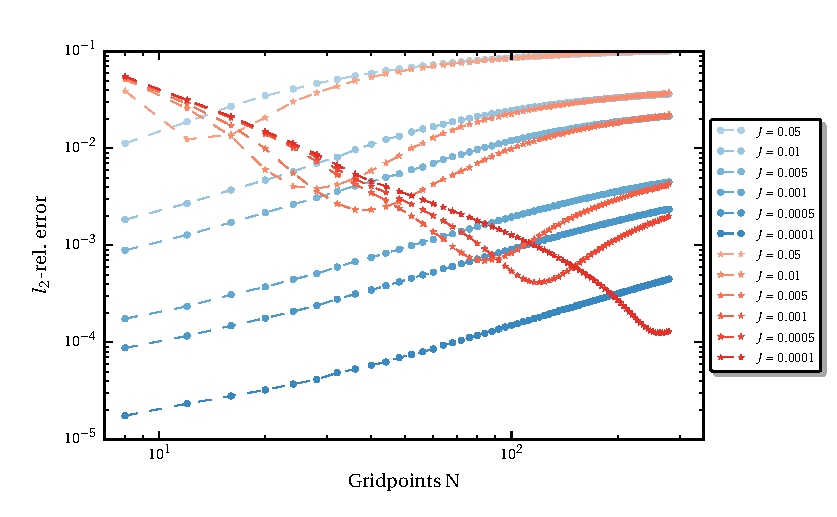
\includegraphics{gfx/immersed_boundary/poiseuille_flow/2_vp/vp_convergence.pdf}\label{fig:vp_conv}
  \caption{Absoluter und relativer Fehler in Abhängigkeit von Dämpfungskonsante $\nu$ und Reynoldszahl $Re$.}
\end{figure}
One can observe again that a decrease in $\nu$  yields a smaller error.
For the second order scheme we can see that with an increase in the resolution, the error increases and finally converges against a constant value.
Even more confusing is the behaviour for the fourth order scheme.
With increasing resolution we can see a decrease into a local minimum, followed by an increase to the same error as the second order scheme.
An explanation of this behaviour can by given by revising the theoretical solution and the finite difference stencils at the immersed boundary.

The error does not converge towards zero, which means there has to be some discrepancy to the theoretical solution.
For a constant $\nu$ there is an offset to the theoretical solution, which we allready saw in figure (REF).
Hence by increasing the resolution the numerical solution converges towards the wrong solution.
The error increases since for a lower resolution, the velocity profile is closer to the assumed theoretical for the second order method.

\begin{align}
 \nu v &= D \frac{\partial^2 v_x}{\partial z^2}  \Rightarrow  v_x = A e^{\sqrt{\frac{\nu}{D}}v_x}
\end{align}
\begin{figure}%
    \centering
    \subfloat[label 1]{{
      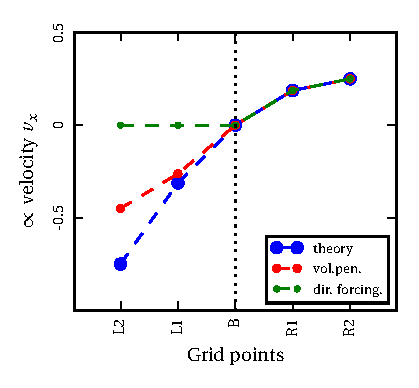
\includegraphics{gfx/immersed_boundary/poiseuille_flow/extra/stencil.pdf}\label{fig:mask_vp}
        }}%
    \qquad
    \subfloat[label 2]{{
      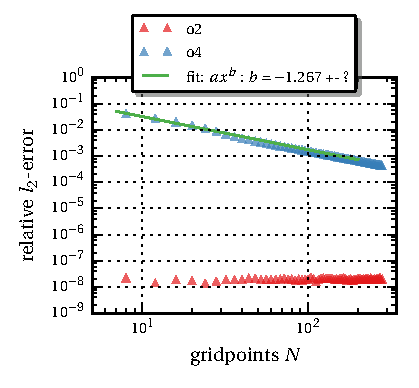
\includegraphics{gfx/immersed_boundary/poiseuille_flow/3_df/relative_l2error.pdf}\label{fig:mask_vp}
        }}%
    \label{fig:example}%
\end{figure}


The explanation for the fourth order convergence has again to do with the discretization error at the boundary.
Figure () shows schematically the velocity profiles for the volume penalizaton method compared to the theoretical.
Due to the different  profiles, the numerical evaluation of the laplace operator results
into different friction rates for the border point \textbf(B), but  also for the first next neighboor in the fluid domain \textbf(R1) when fourth order schemes are used.
For the fourth order scheme the laplace operator at the boundary evaluates to a slightly (CALCULATE) negative value), which means the friction at the boundary due to
viscosity is stronger. The result is a smaller velocity profile which when increasing the resolution starts to overlap best with the theoretical solution at the minimal error.
Finally when increasing the resolution further the error increases since the method converges towards the same resolution as the second order scheme (IMAGE MAYBE?).
An attempt has been made to fit the numerical solution to a quadratic profile for the comparision to a theoretical solution but this didn't work due to blabla
(FIT IDEA NOT WORKING CONVERGENCE AGAINST HIGH RESOLUTION.

\subsection{Direct Forcing Method}

For the comparsion to the direct forcing method another grid convergence study was carried out.  As a parameter we used same as above, the results are shown in figure X.
-We can see o4 not working reason is the same as we can se in figure n) , the laplacian is wrong caclulated at the point B.
As a results an error is induced at the boundaries of the domain.
The second order scheme works perfectly as we compare it to the default implementation.

\subsection{Poiseuille Flow with variable pressure gradient}

Finally

\begin{align}
\frac{\partial p}{\partial x} &= P_0 \sin(\pi n z)
\end{align}

solution with the same non-dimensionalization yields

\begin{align}
 \nu v &=  \sin(\pi n z)
\end{align}

with the condition

\begin{align}
 P_0 &= -\frac{\pi^2n^2}{Re}
\end{align}

to satisfie $v_{max} = 1$.


\begin{align}
 \nu v &= D \frac{\partial^2 v_x}{\partial z^2}  \Rightarrow  v_x = A e^{\sqrt{\frac{\nu}{D}}v_x}
\end{align}
\begin{figure}%
    \centering
    \subfloat[label 1]{{
      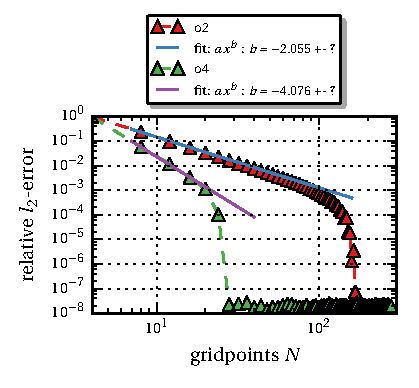
\includegraphics{gfx/immersed_boundary/poiseuille_flow/4_sine/relative_l2error.pdf}\label{fig:mask_vp}
        }}%
    \qquad
    \subfloat[label 2]{{
      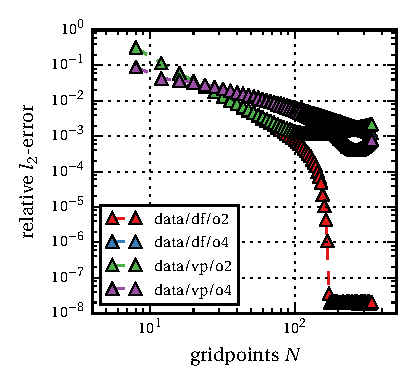
\includegraphics{gfx/immersed_boundary/poiseuille_flow/4_sine/relative_l2error_methods.pdf}\label{fig:mask_vp}
        }}%
    \label{fig:example}%
\end{figure}

\newpage
\subsection{Hagen-Poiseuille Flow}

\subsubsection{Theoretical description}

In the previous testcase the channel walls were aligned parallel to the simulation grid, hence no further interpolation procedures
were necessary. In order to test the accuray of the interpolation methods, we now introduce a testcase with a curved geometry.
Furthermore we have the possibility to investigate the error of non-interpolating methods on curved surfaces.\\
The most simplest extension of the planar poiseuille flow, is the laminar flow through a pipe,
also referred to as Hagen-Poiseuille flow. The setup of the fluid domain is schematically shown in figure ().
We consider a flow in z-Direction where the total size of the simulation domain is set to $L_x = L_y = L$.
The immersed boundary is restricted by a wall at the radius $r_0=0.4L$ where r is defined as the distance from the pipe center $\vec{m} = (L/2, L/2)^T$.
The length $L_z$ can be chosen arbitrary due to the flow invariance in z direction.\\
\begin{figure}[!bp]
  \centering
  \includegraphics[width=0.8\textwidth]{gfx/immersed_boundary/val_volpen/poiseuilleflow.png}\label{b}
  \caption{Theoretical setup of the poiseuille-flow channel.}
\end{figure}
For an analytical solution of this problem we referr to [CITEFLUID].
Once again we can assume a steady state flow which implies $\partial v_z/\partial t = 0$. With the introduction of cylindrical coordinates $(r, \phi, x)$
and the assumption that the flow is independent of $\phi$ the equation of motion reduces to
\begin{align}
        0 &= - \frac{\partial p}{\partial x}  +  \frac{\nu}{r}\frac{\partial}{\partial r}\left(r\frac{\partial u}{\partial r}\right)
\end{align}
The solution is obtained by seperation of variables and integrating twice.
\begin{align}
    u &= \frac{r^2}{4\nu}\frac{\partial p}{\partial x} + A \ln r + B
\end{align}
By using the boundarie conditions $u(r_0) = 0$ and choose the same non-dimensionalization as in section (), with the expection of setting the length scale to $r_0$,
the velocity profile for the channel is given by
\begin{align}
    u &= \frac{r^2 - r_0^2}{4}\frac{\partial p}{\partial x}Re
\end{align}
Since $v_{max} \stackrel{!}{=} 1$ by definition, the pressure condition for the domain needs to be set to
\begin{align}
    \frac{\partial p}{\partial x} = -\frac{4 r_o^2}{Re}
\end{align}

\subsubsection{Grid Convergence Study}

For an error evaluation a grid convergence study was performed, for a constant reynolds number of $Re=100$.
The number of grid points was varied in the intervall $N\in[32, 256]$ with a stepsize of $\Delta N = 16$, furthermore a
simulation with a resolution of $N=512$ was carried out.\\
Since the maximum velocity of the channel is given by $v_{max}=1$, due to the choice of non-dimensionalization,
the sound speed was set to $c^2 = 100$ to fullfill the incompressibilty condition $Ma = v/c < 0.1$. \footnote{In order to exclude
any influence of choice of the sound speed on the resulting error, further simulations were carried out with a diffent $c^2$ and will be discussed}
With this choice the cfl-condition for the system is given by $\Delta t < \min(\Delta x^2 \cdot Re, \Delta x / 10)$.
The resulting timestep for the highest resolution is $\Delta t = 1e-4$.
With the above defined setup all methods introduced in section were tested, for second and fourth order finite difference stencils.\\
For the penalization method the non-dimensionalized damping was set to $J=1e-4$.
It would be possible to choose a larger time step for the lower resolution cases, which means that in general
one would apply a smaller damping rate $J$ in a case of applicaton. To remain consistent in the error convergence, here $J$ and
therefore $\Delta t$ was not altered.\\
The results of the computation are shown from figure () to figure().
In figure (X) the relative $l_2$-error is shown for the volume penalization method with and without the volume fraction method
for second and fourth order. The modified volume fraction method is not present since the computed error is almost identical to the default method,
such that the values overlap in the plot.

\begin{figure}[!pt]
  \centering
  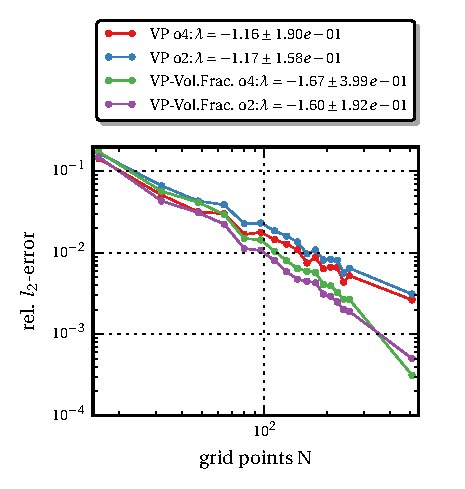
\includegraphics{gfx/immersed_boundary/hpflow/theo/vp.pdf}\label{fig:hpflow_vpgc_theo}
  \caption{blabla}
\end{figure}

\begin{figure}[!pb]
  \centering
  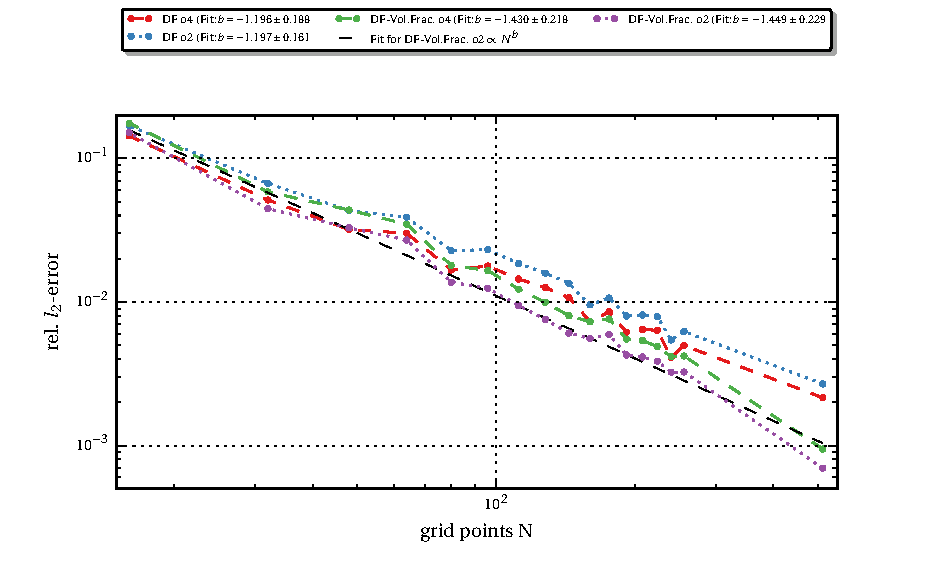
\includegraphics{gfx/immersed_boundary/hpflow/theo/df.pdf}\label{fig:hpflow_dfgc_theo}
  \caption{blabla}
\end{figure}


\begin{figure}[!pt]
  \centering
  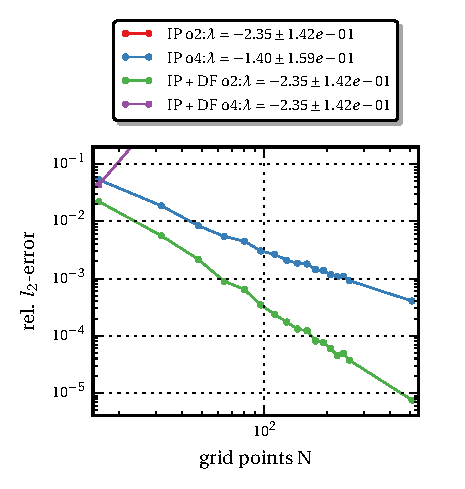
\includegraphics{gfx/immersed_boundary/hpflow/theo/ip.pdf}\label{fig:hpflow_ipgc_theo}
  \caption{blabla}
\end{figure}

\begin{figure}[!pb]
  \centering
  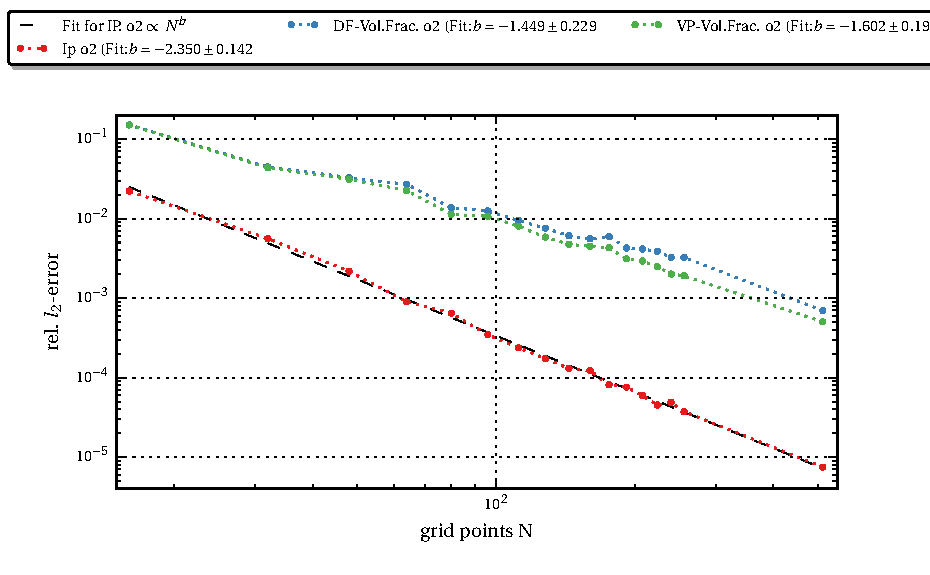
\includegraphics{gfx/immersed_boundary/hpflow/theo/all.pdf}\label{fig:hpflow_allgc_theo}
  \caption{blabla}
\end{figure}

\newpage


For all methods an approximately linear decrease  can be observed.
The error decreases from the order $1e-1$ for low resolutions until


-numerical setup resolution
-sound speed squared
-dt choice
-nu choice

-discussion c2 400

\subsubsection{Long-Term Simulations}
\newpage


\subsection{Taylor-Couette Flow}

-introduction

\subsubsection{Theoretical description}

blub blub

\part{Application}
\chapter{Inertial Waves in a Rotating Cone}

\section{Introduction}

Following the introduction and validation of the immersed boundary methods
we now want to exemplarly investigate a fluid system using these methods
and find out if we can reproduce some of the expected physical properties.
In relation to the research focus of the geophysical fluid mechanics research group, there are a variety
topics of interest.
One area of research lies in the exploration of dynamo effects in geological and stellar system.
In particular this means the generation of magnetic fields by electrically conducting fluids on large scales.
In this thesis we will not consider MHD-equations.
However in general it is considered that the helicity of a fluid domain $\Omega$, given by

\begin{align}
    \int_{\Omega}\dif V  \vec{u} \left( \nabla \times \vec{u} \right)
\end{align}

is directly linked to dynamo action \citep{moffat1978}.
Therefore it would be interesting to find a system which exhibits a large helicity,
as a possible candidate for future researches of the geo dynamo.
Furthermore we are interested in the propagation of inertial waves in different fluid domains.\\
The systems we want to study in this thesis is given by a librating cone, which is compared to
a librating frustum, by inserting a bottom plate into the apex.
Interial waves are excited by a temporal modulation of the rotation frequency.
The objective is to examine the ability to generate inertial modes or wave attractors.
Furthermore we want to study the properties of the helicity of the system and investigate the
decay of inertial oscillations.\\
In this chapter we will use linearized equations. Due to the axial symmetry with the rotating axis,
this problem could be reduced to two dimensions.
However, we want to test the code in a three dimensional setup.
One reason for this is a possible future application of the setup.
This objective would be to study the decay of turbulence in the apex of the cone,
a 3d simulation can not be avoided in this case.



\section{Inertial Waves in a Librating Cone}
\label{cone:theorie_exp}

\subsection{Theoretical Description}

We beginn with a short theoretical description of the problem adapted from \citep{Greenspan1969}, \citep{Beardsley1970}.
For the cone we make the comparsion to the two-dimensional case of a wedge.
This system is based on the idea to introduce a geometric shape, containing a singularity.
Here we want to discuss the propagation of an inertial wave emitting at one of the upper edges of
the wedge as shown in figure \ref{cone:theorie}.
The wave propagates under the angle $\theta = \arccos(\omega/2)$, with respect to the horizontal axis.
We consider an inviscous fluid.
For each reflection the propagation angle with respect to the rotation axis is preserved.
In the case of $\theta<\alpha$ we have a supercritical reflection,
thus a downward traveling wave ray is reflected downslope.

\begin{figure}[!bp]
  \begin{minipage}[c]{0.6\textwidth}
      \centering
        \resizebox{0.7\textwidth}{!}{
       \import{gfx/cone//}{cone.pdf_tex}
      }
  \end{minipage}
  \begin{minipage}[c]{0.3\textwidth}
      \caption{
          Propagation of an inertial wave emitted from the top edge of a wedge,
           where $\Theta$ indicates the direction parallel to the group velocity
            $\vec{c_g}$, s $L$ and $L^{\prime}$ are the path lengths before and after a reflection.
      \label{cone:theorie}
      }
  \end{minipage}
\end{figure}

As a results the wave ray travels towards the lower vertex of the wegde.
It can be shown from the reflection properties given by equation () and (),
that the time for a wave ray to travel the path between two reflections is constant \citep{Beardsley1970},
which is

\begin{align}
    \frac{L}{|\vec{c}_g|} = \frac{L^{\prime}}{|\vec{c^{\prime}}_g|}
\end{align}

This means that the overall propagation time into the apex of the cone becomes infinity, along with the energy density and the wave number.
In conclusion it follows that since no reflection out of the cone apex can occur, the possibilty of inertial modes is not given.\\

\subsection{Experiment}

In order to test these theoretical assumptions  an experimental study was performed by \citep{Beardsley1970}.
The schematic setup of the experiment is shown in figure \ref{cone:setup_experiment}.\\
In the first part of the experiment a plexiglass cylinder, containing a conical shaped cavity,
of height $H=\SI{19.95}{\centi\meter}$ and a radius of $r=\SI{19.95}{\centi\meter}$ was used.
The apex half angle was set to $\alpha=24^{\circ}3.7^{\prime}$ degree.
For the rotation rate a frequency of $\omega =\SI{6.28}{\radian\per\second}$ was chosen.
As a fluid, water was used, the resulting viscosity, given by \citep{tipler2003}, is $\nu = \SI{1.0}{\milli\pascal\second}$.
The resulting Ekman number is

\begin{align}
    \Ekman = \frac{\nu}{\omega r H^2} \approx 7.72\cdot 10^{-6}
\end{align}

In order to exite inertial waves the cone is librating.
The total rotation rate is given by

\begin{align}
\Omega(t) = \Omega_0 + \epsilon \omega \cos(\omega t)
\end{align}

where $\omega$ is the libration frequency.
This means that excitation mechanism results from wall friction, induced
by a modulation of the constant rotation frequency $\Omega_0$.

\begin{figure}[!bt]
      \centering
        \resizebox{0.6\textwidth}{!}{
       \import{gfx/cone///}{experiment.pdf_tex}
      }
      \caption{
      experiment
      \label{cone:setup_experiment}
      }
\end{figure}

For the analysis the dynamic pressure field was measured at at different depths along the rotation axis,
with the libration frequency in the range of $0.25\leq\omega/2\Omega\leq2$.
The pressure and phase lag spectrum, for each measurement height, show that for this setup
no inertial modes can be observed.\\
In the second part of the experiment the apex of the cone was replaced by a frustum through the
insertion of a bottom plate in the cone, at the position $z/H = 0.261$.
With this setup yields the possibility that a wave ray can be reflected on bottom of frustum.
The pressure and phase lag spectrum in this setup show that
independent of the height resonances occur which can be associated with standing waves.
Hence inertial modes exist.

\section{Numerical Implementation of Libration}

For the numerical implementation of the experiment, we will use a modified set of the equations
introduced in section \ref{THEORIE:ROT}.
We have to concern that the system has now a time-depent rotation rate.
For the non-dimensional system, with $\vec{u}^* =  \vec{u} (|\vec{\Omega}|L)^{-1}$, we set

\begin{align}
    \vec{\Omega(t)} = 1 \; + \; \epsilon \cos(\omega t)\vec{e}_z
\end{align}

There are two options, which should be considered here.
First of all, we can choose a rotating coordinate system with a constant velocity $\Omega_0$.
This means the we can directly use the equations () to (). Since the overall rotation rate of the system is
modulated, it is necessary to introduce the boundary conditions

\begin{align}
    \vec{v}|_{Border}  = \Omega \times \vec{r} = \begin{pmatrix}
           -y \epsilon \cos(\omega t) \\
           x \epsilon \cos(\omega t) \\
           0\\
         \end{pmatrix}
\end{align}

However, obtaining a linearized version of the boundary methods is not as easy.
In addition we think it is safer to use No-Slip boundaries with zero velocity, as
the taylor-couette system showed that other boundarie velocities can create a larger numerical error.
The alternative option is the introduction of an accelerated frame of reference.
In this case the boundary conditions do not need to be modified, but the coriolis forcing term is given by \citep{Tilgner2007}.

\begin{align}
    \vec{f} &= 2 \vec{\Omega} \times \vec{v} + \pdn[]{t}\left(\vec{\Omega} \times \vec{v} \right)
            = \begin{pmatrix}
           -y \omega \epsilon \cos(\omega t) \\
           -x \omega \epsilon \cos(\omega t) \\
           0\\
         \end{pmatrix}
            + 2\begin{pmatrix}
           - ( 1 + \epsilon \sin(\omega t)v_x \\
             ( 1 + \epsilon \sin(\omega t)v_y \\
           0\\
         \end{pmatrix}
            = \begin{pmatrix}
           -y \epsilon \cos(\omega t) \\
           -x \epsilon \cos(\omega t) \\
           0\\
         \end{pmatrix}
\end{align}

In the last step the linearization was introduced.
Finally the non-linear advection term was removed from the equations of motion, which
are then given by

\begin{align}
    \label{theorie:rotns}
    \pdn[u]{t} = -c^2\nabla \rho + \Ekman \Delta \vec{u} + \vec{f} \qquad;& \qquad  \nabla \vec{v} = 0
\end{align}

Finally one additional stability criterion shall be introduced,
It is important that the time for propagting information from on side of the domain
to the other, is much smaller than the overall rotation rate.
\footnote{Private communication with A. Tilgner}
Since information inside the fluid domain propagates at an artificial sound speed,
this yields the estimation

\begin{align}
    t = \sqrt{\frac{2}{c^2}} << 2\pi
\end{align}

A good estimation is given by setting $c^2 = 500$.
It could be observed that otherwise, not only physical wrong results are obtained but also
numerical instabilitys can occur.
\footnote{Private communication with O. Goepfert}
\newpage

\subsection{Setup}

This section introduces the setup which has been used for the simulations presented in this chapter.
Figure \ref{cone:setup_image} shows the geometry of the fluid domain. The parameters are given by

\begin{multicols}{2}
\begin{description}
    \item[$H$]{Total height of the simulation domain}
    \item[$h_c$]{Height of the Cone}
    \item[$h_t$]{Height of the bottom plate for a frustum}
    \item[$r$]{Radius of the bottom plate}
    \item[$O$]{Offset at the top of the Cone}
    \item[$\alpha$]{Slope of the Cone}
    \item[$\Omega$]{Rotation rate}
    \item[$\omega$]{Frequency of the libration}
    \item[$\epsilon$]{Amplitude of the libration, default is 1\footnote{linear}}
\end{description}
\end{multicols}

This convention will be used throughout rest of this chapter.
For the implementation the testcase function template introduced in chapter () is used.
The use of the different parameters with this template is shown in Appendix ().

\begin{figure}[!bp]
  \centering
        \resizebox{0.6\textwidth}{!}{
       \import{gfx/cone/conesim//}{setup.pdf_tex}
      }
      \caption{Numerical Setup for the Simulations \label{cone:setup_image} }
\end{figure}
\clearpage

\section{Data Analysis}

The main interest, in the analysis of the simulation data, lies in the identification of possible inertial modes.
A appropriate choice is to consider the energy in the $v_z$ velocity component of the intertial mode,
which is given by

\begin{align}
    \left<v_z^2 \right>(t) =  \int \dif V v_z(t)^2 \approx \sum_{i, j, k}^{N_x,N_y,N_z} \Delta x \Delta y \Delta z \left.v_z(t)^2 \right|_{i,j,k}
\end{align}

This has multiple benefits

\begin{itemize}
    \item The $v_z$-velocity component is indepent of the coordinate system which is used, it is not necessary
                to compute a transformation to inertial frame.
    \item The energy induced by the libration is perpendicular to this component, thus all components
            in the $v_z$-component are created by inertial  wave propagation(umshr)
\end{itemize}

In figure \ref{fig:cone:cyl_vzmode}, this energy is shown exemplarly for two libration frequencies for a cylinder.
\footnote{From section so und so}
For a resonance of the system ($\omega=1.2$) it takes further time until a steady state, with a constant oscillation is reachd.

\begin{figure}[!pb]
  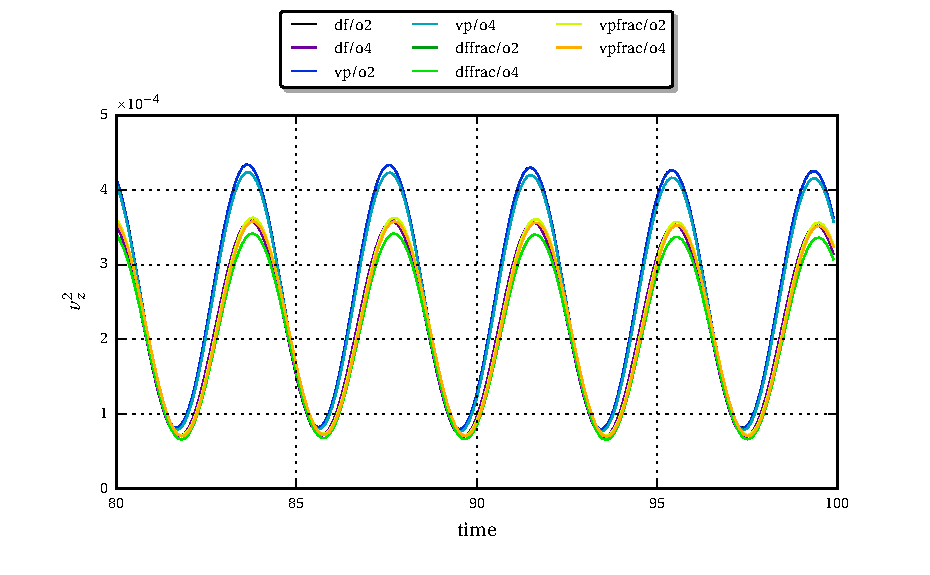
\includegraphics{gfx/cone/cylinder/cyl_vz.pdf}\label{fig:cone:cyl_vzmode}
  \caption{Kinetic energy in $z$-direction for the direct forcing second-method and $\omega=1.2$.}
\end{figure}
\clearpage

In order to obtain a spectrum, the energy amplitude is computed from the last two extrem of $<v_z^2>$.
\begin{align}
    A\left(\left<v_z^2\right>\right) = \frac{\max(\argmax(\left<v_z^2\right>_{v})) - \max(\argmin(\left<v_z^2\right>_{v}))}{2}
\end{align}

We estimate the error of this method of order $\sigma 5-10A$.(Wie schreiben?)
For resonances the error is more likely to be in the range of 10 \% for non 5\%.
This can also be seen in figure ().\\
Secondly we want to compute the helicity of the system.
Here we use the normalized helicity, given my  \citep{XXX}

\begin{align}
H(t) = \frac{\int_V \dif V \vec{v} (\nabla \times \vec{v})}{\int_V \dif V |\vec{v}||\nabla \times \vec{v}|}
 = \frac{\sum_{i,j,k=0}^{N_x, N_y, N_z} \vec{v}_{i,j,k} (\nabla \times \vec{v}_{i, j, k})}
 {\sum_{i,j,k=0}^{N_x, N_y, N_z}|\vec{v}_{i,j,k}|| \nabla \times \vec{v}_{i, j, k}|}
\end{align}

The discretization of the rotation operator is using a central difference of second order.



\section{Simulation of a Librating Cylinder}
\label{cone:sec:lib_cylinder}

As a first step towards the implemenation of the librating cone,
simulations of fluid flow in a librating cylinder were carried out.
Despite the the theoretical and experimental results, discussed in section \ref{cone:theorie_exp},
it is diffult to find results in literature which would be suitable for an appropiate validation for the cone.
For the cylinder on the other hand, theoretical and numerical results are available.\\

\subsection{Setup}

The simulations were performed for all immersed boundary methods introduced in chapter \ref{IBM}.
Due to a misunterstanding the aspect ratio of the cylinder was set to $\Gamma=r/H=\nicefrac{0.5}{1.1}$ instead of $\frac{1}{2}$.
The main simulation parameters are given by

\begin{center}
\vspace*{0.7ex}
\begin{tabular}{c|c|c|c|c|c|c|c }
 $\leftarrow  \omega \rightarrow $ & $\Gamma$ & $\Delta t$ & $\Delta x$ & $c^2$ & $\Ekman$  & $l_x, l_y, l_z$ & $T_{end}$\\
\hline
 $[0.2,\; 2], \Delta w = \nicefrac{1}{10}$ & $\nicefrac{0.5}{1.1}$ & $10^{-4}$ & $\nicefrac{1}{128}$ & 500 & $10^{-4}$  & (1.1, 1.1, 1.1) & 100\\
\end{tabular}
\vspace*{0.7ex}
\end{center}
\newpage

\clearpage

\begin{figure}[!t]
  \centering
  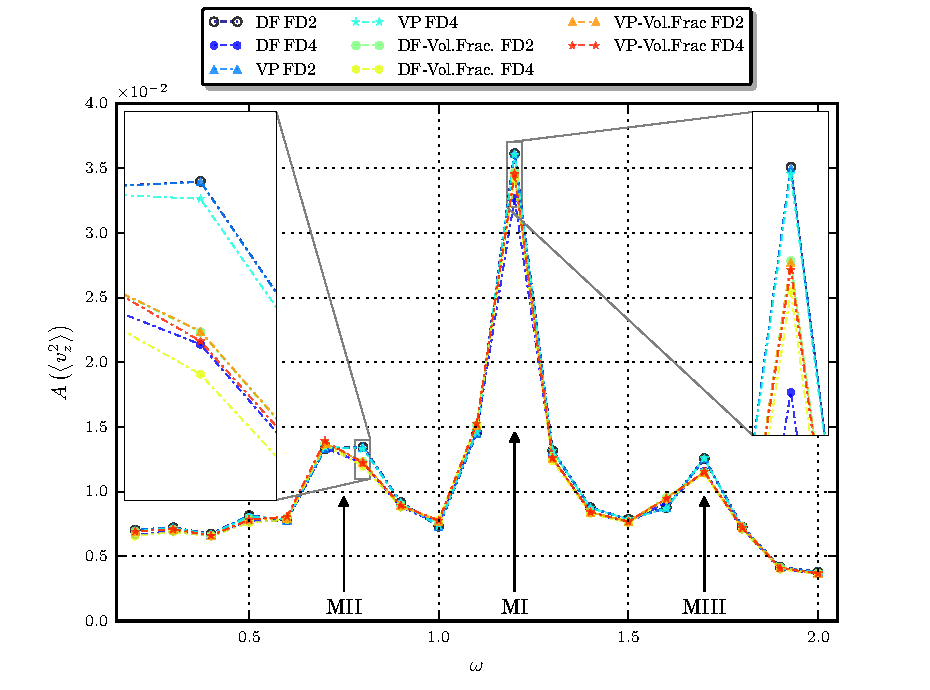
\includegraphics{gfx/cone/cylinder/cylinder.pdf}  \caption{\label{fig:cone:cyl}
    Amplitude of the kinectic energy of $v_z$, as function of the liberating frequency $\omega$,
   for the direct forcing (DF), volume penalization (VP) method with or without Volume Fraction and
      second and fourth order (o2/o4) finite differences.}
\end{figure}

\bgroup\large
\begin{table}[!b]
\centering
\def\arraystretch{1.5}%
\begin{tabular}{c c c c c}\toprule
            &    m =  1  & m = 2   &    \\ \hline
\midrule
        n=1 &   0.698433         &              0.398913 &    \\
        n=2 & \cellcolor{blue!25}  1.195232         &        \cellcolor{blue!25}      0.754094 &    \\
        n=3 &   1.490715         &              1.042313 &    \\
        n=4 &  \cellcolor{blue!25} 1.660912         &     \cellcolor{blue!25}         1.262759 &    \\
        n=5 &   1.762270         &              1.426587 &    \\
        n=6 &   1.825743         &              1.547435 &    \\ \hline

\bottomrule
\label{cone_cyleigenvalues}
\end{tabular}
\caption{Eigenvalues of the (n, m)-inertial modes in  a cylinder with aspect ratio $\nicefrac{5}{11}$.
            Possible modes are highlighted.}
\end{table}
\egroup
\clearpage

\subsection{Results}
\subsubsection{Inertial Wave Spectrum}

For all simulations, the kinetic energy of the $v_z$ velocity component was computed.
The results for the computation of the amplitude $A\left(\left<v_z^3\right>\right)$, in dependcy of the libration
frequency are shown in Figure \ref{fig:cone:cyl}.
All methods which were used show a similar profile.
The largest amplitude deviations can be spotted at a frequency of $\omega=0.8$ and are of the order $\approx2\cdot10^{-3}$.\\
It can be noted that a large resonance  occurs at the position $\omega=1.2$ of the order $\approx3.5\cdot10^{-2}$, followed by two
smaller resonances at $\omega=0.75$ and $\omega\approx1.7$ of order $\approx1.3\cdot10^{-2}$.
To make the deviations between the methods more visible, two inset plots are shown
set to the location $\omega=0.8$ and $\omega=1.0$.\\
For both positions, the largest amplitude is given by the direct forcing method of second order, followed by
the volume penalization method of second and fourth order.
The amplitude difference betweens the first two methods is just slighty visible when looking at the right inset plot.
It seems like these three methods yield nearly the same results for alle frequencies.
For all remaining methods  no strict order or grouping can be recognized.\\
The results for the interpolation method are not plotted in this spectrum, since the simulations became numerically unstable.

\subsubsection{Eigenvalues for the inviscid equations}

For a comparison to the theoretical solution introduced in section \ref{numerik:rotatingoderso}
the eigenvalues for the (n, m)-inertial modes with $n\in[1,6]$ and $m\in[1, 2]$ were  computed.
The results are shown in table \ref{cone_cyleigenvalues}.
There are four possible canditates,  which could correspond to the peaks in the spectrum.
The largest peak at $\omega=1.2$ is close to the eigenvalues of the (1, 2) and (2, 4) mode.
The left peak at $\omega=0.75$ could be the (2, 2) mode,
whereas the peak on the right side at $\omega=1.7$ is close to the eigenvalue of teh (1, 4) mode (evlt. M1 M2 M3 defi).
The eigenvalues for even $n$ are not considered. Due to the libration mechanism only azimuthal velocity fields which are even,
in relation to the plane $z=H/2$ are possible \citep{Sauret2012}.
Furthermore we are not considering modes with $m\geq2$. These modes are allready not visible at an Ekman number of $5\cdot10^{-5}$,
due to viscous damping of large wavenumbers \citep{Sauret2012} .

\subsubsection{Helicity}

The computation of the helicity was splitted into an integral over the upper and lower half
of the cylinder.  A result for $\omega=1.5$ is exemplarly shown in figure \ref{cone:cyl_helicity}.
In the upper half of the cylinder a negative helicity can observed, the maximum of the amplitude is of order $10^{-1}$.


\clearpage
\begin{figure}[!t]
  \centering
  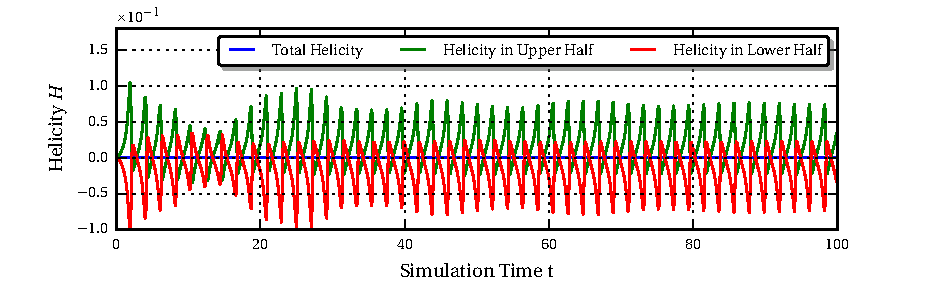
\includegraphics{gfx/cone/cylinder/helicity.pdf}  \caption{
      Time-depent Helicity for $\omega=1.5$. The direct forcing method of second order was used.
      \label{cone:cyl_helicity}
      }
\end{figure}
\begin{figure}[!p]
  \centering
  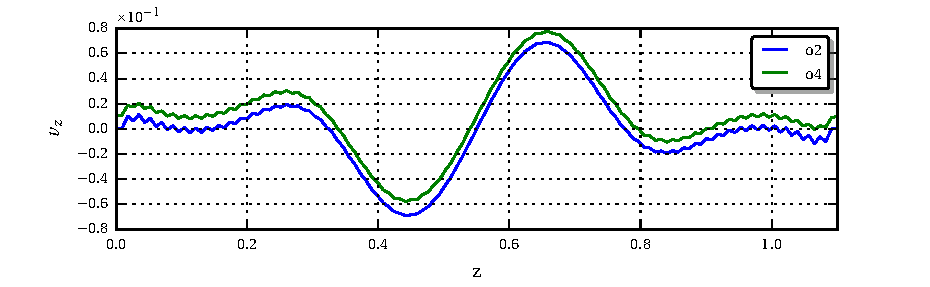
\includegraphics{gfx/cone/cylinder/oscillations.pdf}  \caption{
      Numerical oscillations on the axis $(x,y) = 0.5, 0.5$ and variable $z$.
      For direct forcing method of second (o2) and fourth (o4) order, at $\omega=1.5$.
      \label{cone:cyl_oscillations}
      }
\end{figure}
\begin{figure}[!b]
  \centering
  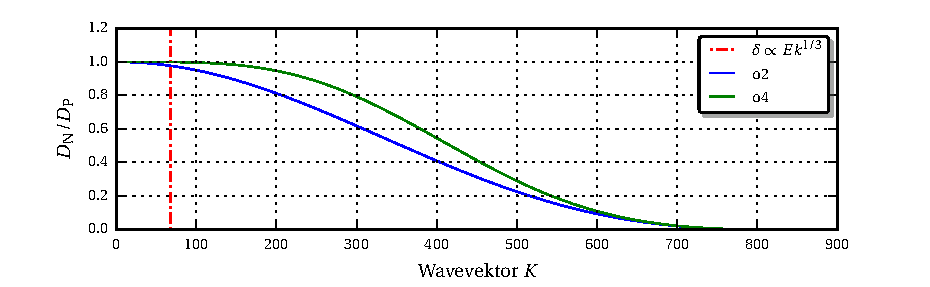
\includegraphics{gfx/cone/cylinder/numvis.pdf}  \caption{
      relative Numerical Viscositiy computed for $\Ekman=10^{-4}$ for 2nd and 4th- order central differencing schemes.
      \label{cone:cyl_numvis}
      }
\end{figure}
\clearpage

In the lower half of the cylinder a positive helicity can observed, the maximum is of the same order as before.
The helicities are symmetric with respect to zero, thus $H_{\text{up.}} = -H_{\text{low.}}$.
As a result, it can be noted that the total helicity of the cylinder evaluates to zero for all times.

\subsubsection{Numerical Oscillations}

For all immersed boundary methods numericall oscillations are observable.
Figure \ref{cone:cyl_oscillations} shows this for the 2nd and 4th order direct forcing method and $\omega=1.5$.
The profile is taken along the $z$-Axis at $(x,y)=(\nicefrac{1}{2},\nicefrac{1}{2})$.
It can be noted that the error is larger in the regions near to the wall.
One important detail is that the oscillations are only observable in $z$-Direction not
in th $(x,y)$ plane.
For the 4th order method an upwinding scheme has been used. In comparison to the second order FTCS-Scheme,
it is visible that the oscillations are slightly dimished.

\subsubsection{Numerical Viscosity}

Finally the ratio between the numerical and physical viscosity was computed, according to equation \ref{THEORIE}.
The results are shown in figure \ref{cone:cyl_numvis}.
The red bar denotes the $K$ vektor for the width of an inertial wave $\propto \Ekman^{1/3.}$
For this value the ratio is $\approx{0.977}$.
For larger wave vektors the 4th order method has a better approximation, than 2nd order.
For both methods a decrease in the numerical viscosity can  be observed.
The largest possible wave vektor of the  system is possible for $\lambda = 2\Delta x$,
it follows that $K_{\text{max}} = \nicefrac{2\pi}{\lambda} \approx 402.1$.
=

\clearpage

\subsection{Discussion}

\subsubsection{Immersed Boundary Methods o Spectrum}

The different immersed boundary methods show similar results in the profile of the amplitudes.
This in agrement with the results of validation testcases of the hagen-poiseuille and
taylor-couette flow, since the discretzation error of the boundaries is roughly of the same order of $\approx?$ (HMM..).
The results from this simulation are not useable for an error estimation however it can be noted

-ipmethod here
- results diskussion ip kaputt \
-keine aussage über die fehler
-nur ipo2 ip o4 etc vergleich
-wie bereits gesehen liegen die fehler für df vpfrac etc in etwe in der gleich größenordnung

-theorie
-tabelle eigenwerte
-paper kurz erklären symetrie warum fehlen bestimmte moden ? ?
\subsubsection{Numerical Oscillations}
-numerical oscilations
\subsubsection{Numerical Viscosity}
-numerical viscosity
\subsubsection{Helicity}
-helic ist 0

An numerical study of the non-linear system was performed by \citep{BLA}, to which the results will be compared.
a comparision between the different IBMs and the detection of numerical errors.

\newpage

\section{Simulation of a Librating Cone}

In this section we will discuss the different numerical simulations, which has been performed
with a librating cone. We begin with the comparison to the experiment performed by \citep{Beardsley1970}.
As a next step we analyse the physical behaviour when performing the transition from a cylinder
to a cone and finally  we will investigate the influence of different offsets on top of the cone.
All simulations performed in this section use the introduced setup with different geometric parameters.
As a IBM we choose the direct forcing  method of second order.

-as a convention we refer to frustom cone etc
-explain method used..
-libration intro immer gleich .. sin etc

\subsection{Simulation of the Experiment}

The setup for this simulation is oriented on the experimental setup given by \citep{Beardsley1970}, which
we disussed in section ().
In the first part of the experiment a plexiglass cylinder of height $H=\SI{19.95}{\centi\meter}$ and a radius of
$r=\SI{19.95}{\centi\meter}$ was used. The apex half angle was set to $24^{\circ}3.7^{\prime}$ degree,
which relates to our setup with $\alpha=65^{\circ}56.3^{\prime}$
For the rotation rate a frequency of $\omega =\SI{6.28}{\radian\per\second}$ was chosen.
As a fluid, water was used, the resulting viscosity,given by \citep{tipler2003}, is $\nu = \SI{1.0}{\milli\pascal\second}$.
The resulting Ekman number is given by

\begin{align}
    \Ekman = \frac{\nu}{\omega r H^2} \approx 7.72\cdot 10^{-6}
\end{align}

In the second part of the experiment the apex of the cone was replaced by a frustum through the
insertion of a bottom plate at the position $z/H = 0.261$.
For the simulation we choose an Ekman number of $\Ekman =  10^{-4}$, since a simulation of higher ekman numbers is
diffcult to realise due to the computational effort.
Furthermore we set $\alpha = \arccos(1/2) = 60^{\circ}$, $H=1$ and $r=0.5$.\\
This means that for $\omega=1$, the propagation of an inertial wave package is parallel to the slope of the cone.
For the offset on top of the cone, we obtain the condition

\begin{align}
    o = H - h_c =  1 - r\tan{\alpha} \approx 0.134
\end{align}

The simulation has two setups in analogy to the experiment.For the second part the bottom plate is set to $h_b=0.25$.
A series of simulations of these systems where performed, with the parameters

\begin{center}
\vspace*{0.7ex}
\begin{tabular}{c|c|c|c|c|c|c }
%\begin{tabular}{p{0.1\linewidth}| p{0.1\linewidth}| p{0.1\linewidth}|  p{0.1\linewidth}| p{0.1\linewidth}| p{0.1\linewidth} }
$ \leftarrow  \omega \rightarrow $ & $\Delta t$ & $\Delta x$ & $c^2$ & \Ekman  & $l_x, l_y, l_z$ & $T_{end}$\\
\hline
$[0.2,\; 2], \Delta w = \nicefrac{1}{10}$ & $10^{-5}$ & $\nicefrac{1}{128}$ & 500 & $10^{-4}$  & (\{1, 0.75\}, 1, 1) & 100\\
\end{tabular}
\vspace*{0.7ex}
\end{center}

\clearpage
%\begin{figure}[!tp]
%  \begin{minipage}[c]{0.6\textwidth}
%      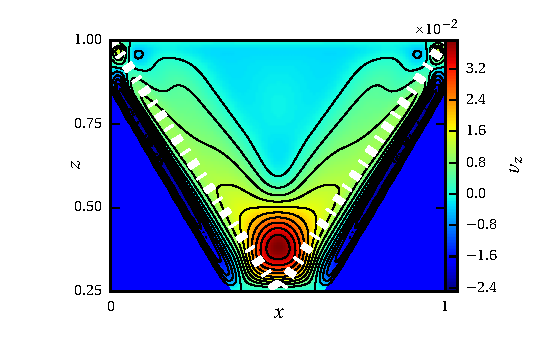
\includegraphics{gfx/cone/experiment/contour.pdf}\label{fig:mask_vp}
%  \end{minipage}\hfill
%  \begin{minipage}[c]{0.3\textwidth}
%  \caption{Stability regions for $\Omega_s$ for different Runge-Kutta methodsi
%    Stability regions for $\Omega_s$ for different Runge-Kutta methodsi
%  }
%  \label{fig:num_rkstab}
%  \end{minipage}
%\end{figure}
%
%\begin{figure}[!tp]
%  \begin{minipage}[c]{0.3\textwidth}
%  \caption{Stability regions for $\Omega_s$ for different Runge-Kutta methods
%  Stability regions for $\Omega_s$ for different Runge-Kutta methodsi
%  }
%  \label{fig:num_rkstab}
%  \end{minipage}
%  \hfill
%  \begin{minipage}[c]{0.6\textwidth}
%      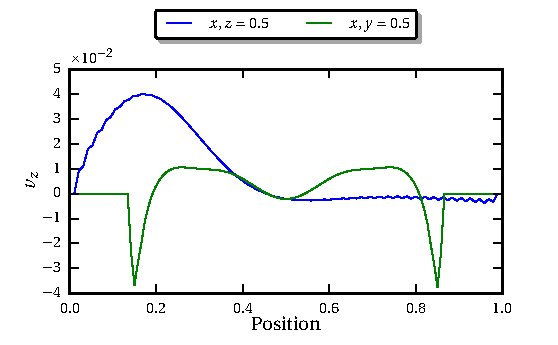
\includegraphics{gfx/cone/experiment/error.pdf}\label{fig:mask_vp}
%  \end{minipage}
%\end{figure}

\begin{figure}[!bp]
  \centering
  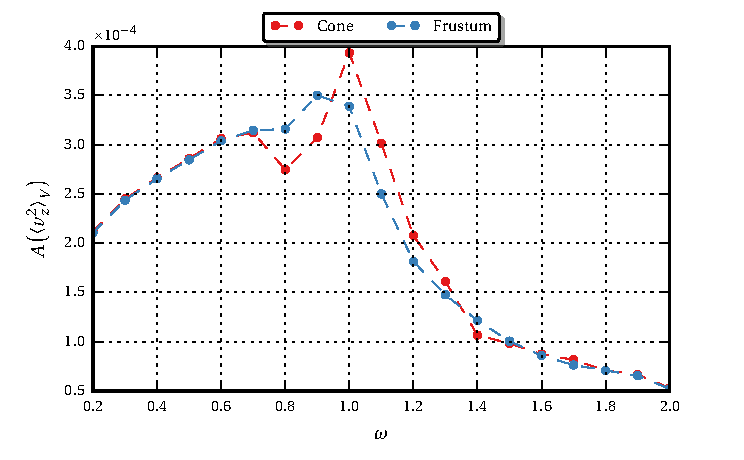
\includegraphics{gfx/cone/experiment/experiment.pdf}
  \caption{Amplitude $A\left(\left<v^2_z\right>_V\right)$ as a function of the libration frequency $\omega$,
            for a cone and a frustum.  \label{fig:cone_expseries} }
\end{figure}

\subsubsection{Results \& Discussion}
\label{cone:exp}

The results of the simulations are shown in figure \ref{fig:cone_expseries}.
For both cases, the frustum and the cone, we can observe an increase in $A\left(\left<v^2_z\right>_V\right)$
from $\approx 2\cdot10^{-4}$ at $\omega=0$ to  $\approx 3.4\cdot10^{-4}$ for the frustum and $\approx 4\cdot10^{-4}$ for the cone,  at $\omega=1$.
From here one the Amplitude decreases to $\approx 5\cdot10^{-5}$ at $\omega=2$.\\
A difference between the two setups can be observed in the surrounding area of $\omega=1$.
For the cone the increase of the amplitude is interrupted at $\omega=0.6$, a minimum can be observed at $\omega=0.8$, followed by
a peak at $\omega=1$. For the frustum the minium is not directly visible but it can be noted that the
amplitude does not increase as much at $\omega=0.7$, as for lower frequencies.\\
The maximum occurs at $\omega=0.9$, in comparison to the cone we see an increase in the amplitude of $\approx 5\cdot10^{-5}$.
However, it has to be considered, that due do the stepwidth of $\Delta \omega = 0.1$, the exact position of the maxima is
not apparent.\\
One possible assumption, regarding the position of the maximum with respect to the frequency, is that
the expansion of the frustum with a tip  results in a shift to lower frequencies.
The left shift in the decrease for $\omega > 1$ furthermore supports this idea.\\
Overall it appears that the (spectrum) can be divided into two domains $\Omega_1~=~\{0\leq\omega<1$\} and $\Omega_2~=~\{1\leq\omega\leq2\}$.
This result is not unexpected, since we choose the slope $\alpha$ of the cone such that for $\omega=1$, it is parallel
do the group velocity $\vec{c}_{g}$.
For $\omega\in\Omega_1$ the results for both setups are similar, since in this domain, the cone tip does not act as an attractor.
An inertial wave propagates the top, after a reflection on the side of the cone.
Hence, for both setups we obtain a similar (spectrum).
The differences occur when $\omega$ is reaching the critical slope, in this scenario an inertial wave propating from the
top edges, travereses directly into the apex of the cone, or is reflected slightly at he bottom plate of the frustum.
As a results we see the increase in the amplitude.
For $\omega\in \Omega_2$ we would expect further reflections for the frustum, however the similar
decay of the amplitude refutes this assumption.\\
The results of the simulation do not match with the ones of the experiment we discussed in section ().
A possible explanation we want to propose here, is the use of a different Ekman number, which is of order $10^{-4}$ in contrast
to the one of the experiment of $10^{-5}$.
As a consequence the width of an inertial wave packet, given by $\propto \Ekman^{1/3} \approx 2\cdot10^{-2}$ (see \citep{} or section...),
is around twice the size as in the experiment. We assume that as a results a wave reflecting on the bottom of the frustum
is strongly damped due to wall friction.
DISCUSS T:\\
damping  could be propt $\Ekman \vec{K}$.

\subsection{Transition to from a Cylinder to a Cone}

We now want to further investigate the results from the previous simulation.
The assumption was made, that the inserted bottom plate is to narrow to support an efficient reflection
of inertial waves, due to frictional losses at the bottom of the cone. Thus, the next objective would be to
test the influence of different gap radii $r$.\\
We propose a setting where we begin with the possible largest bottom gap, which is $r=0.5$.
As a next step we iteratively decrease the size of the gap by $\Delta r = 0.125$ until $r=0$ is reached.
An alternative approach to this woudld be to change the offset from the bottom of the cone, which would result in a constant
slope but different heights of the simulation domain.
The influence on the simulation domain is shown in figure ()(b).
For $r=0.5$ the domain is given by a cylinder, which than transforms into a cone with a frustum and finally with an apex for $r=0$.
The main simulation parameters are given by

\begin{center}
\vspace*{0.7ex}
\begin{tabular}{c|c|c|c|c|c|c|c }
%\begin{tabular}{p{0.1\linewidth}| p{0.1\linewidth}| p{0.1\linewidth}|  p{0.1\linewidth}| p{0.1\linewidth}| p{0.1\linewidth} }
$\leftarrow r \rightarrow$ & $ \leftarrow  \omega \rightarrow $ & $\Delta t$ & $\Delta x$ & $c^2$ & \Ekman  & $l_x, l_y, l_z$ & $T_{end}$\\
\hline
$[0,\; 0.5], \Delta r =0.125$ & $[0.2,\; 2], \Delta w = \nicefrac{1}{10}$ & $10^{-5}$ & $\nicefrac{1}{128}$ & 500 & $10^{-4}$  & (1, 1, 1) & 100\\
\end{tabular}
\vspace*{0.7ex}
\end{center}
%
%\subsubsection{Results \& Discussion}
%\begin{figure}[!bp]
%      \begin{minipage}[c]{0.4\textwidth}
%      \centering
%        \resizebox{0.8\textwidth}{!}{
%       \import{gfx/cone/transition//}{attractor.pdf_tex}
%      }
%      \end{minipage}\hfill
%  \begin{minipage}[c]{0.6\textwidth}
%      \caption{
%          Wave attractor in a cylinder $\left(\text{\colorbox{green}{\textcolor{green}{o}}{\null}}\right)$
%          and shifted\\ attractor $\left(\text{\colorbox{red}{\textcolor{red}{o}}{\null}}\right)$
%          for $r<0.5$. To maintain the same attractor the point of reflection has to be at the same height $h_r$.
%      }
%      \label{cone:theorie}
%      \end{minipage}\hfill
%\end{figure}



\subsubsection{Results \& Discussion}

The results of the simulations are shown in figure \ref{fig:cone:transition}.
For $r=0$ we can see the inertial modes of a librating cylinder, which is in accordance
to the results we discussed in section \ref{cone:sec:lib_cylinder}.
With an decrease of the radius we can observe a change in the position and amplitude of the
inertial modes. We want to exemplarly discuss this pattern for the (2, 2) mode at $\omega=1.3$, where it is the best visible.
For all other modes the transition results in a similar behvavior.\\

\begin{figure}[!pt]
  \centering
  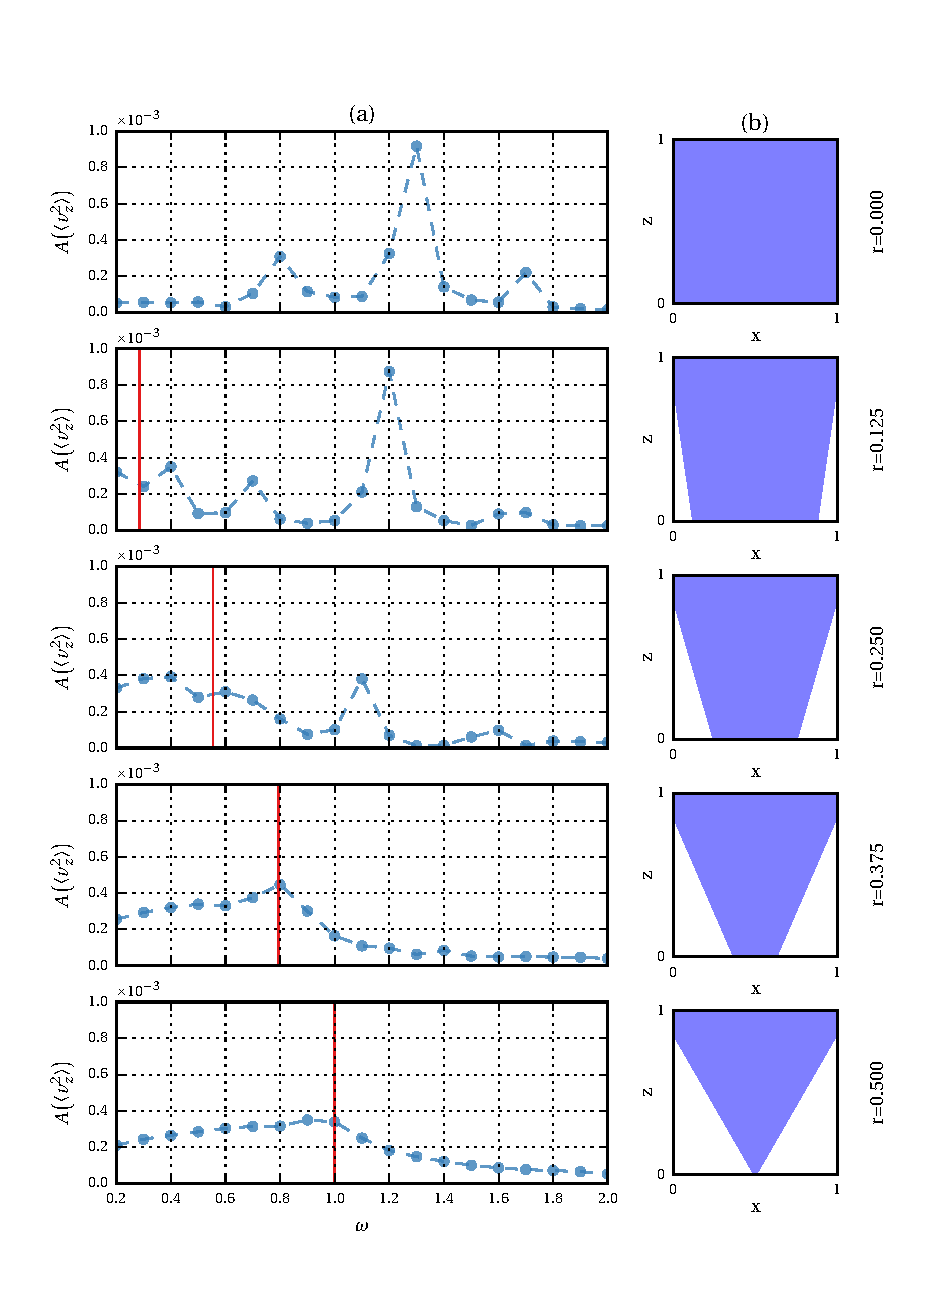
\includegraphics{gfx/cone/transition/transition.pdf}
  \caption{\label{fig:cone:transition}
    Simulation of
  }
\end{figure}

The decrease of the radius leads to a shift to lower frequencies of the (2, 2) mode,
from $r=0$ to $r=0.375$ it is of the order $\Delta \omega=0.1$.
Furthermore we can see, that during the transition a damping of the mode occurs.
For $r=0.5$ the amplitude is of order $\approx8.9\cdot10^{-3}$, for $r=0.375$ it is
$\approx8.9\cdot10^{-3}$ and for $r=0.25$ we obtain $\approx3.8\cdot10^{-3}$.\\
Whereas the first decrease of the radius does not significantly affect the amplitude,
the second decrease leads to a strong damping to less than half of the original size.
With a further decrease in $r$, the (2, 2) mode is annihilated.
\footnote{ for the possible (1, 2) mode we still can observe a slight increase of the amplitude at $r=1.4$}
One possible explanation for the shift can be given
by having a look at the inertial mode structure, for different radii as shown in figure \ref{fig:cone:phase}.\\
For $r=0.5$ we have an inertial mode, which is symmetric to the plane $h/2$.
In this plane, the waves excited from the bottom and top of the cylinder, annihilate each other and form a wave node.
An decrease of radius breaks the axial symetrie of the inertial mode.
As a result only a distorted version of the mode can exist, where the center of the wave node
is given by the intersection of the diagonals from the top to the bottom edges of the frustum.
In order to obtain the new shape it is necessary to increase the propagation angle $\Theta$,
which is equivalent to lowering the libration frequency.
We can furthermore say that for $r \rightarrow 0$, the center given by

\begin{align}
c  = r \frac{h}{r+\nicefrac{l_x}{2}}
\end{align}

converges against zero, hence a mode cannot exist in this state.
Beside the changes of the inertial modes it can be noted, that simultaneously to the decrease of the radius,
a lift of the amplitudes at lower frequencies occurs.
The vertical lines in figure \ref{fig:cone:transition} are set to the position $\omega=\Theta$.
The area $\omega<\Theta$ can again be associated with the frequency domain, where the wave propagation angle $\Theta$ is larger than
the  slope of the cone $\alpha$ and waves propgate to the top, up on reflection on the slope.
For $r=0$ we have the indentical setup to the simulation in section \ref{cone:exp}.

\begin{figure}[!pt]
  \centering
  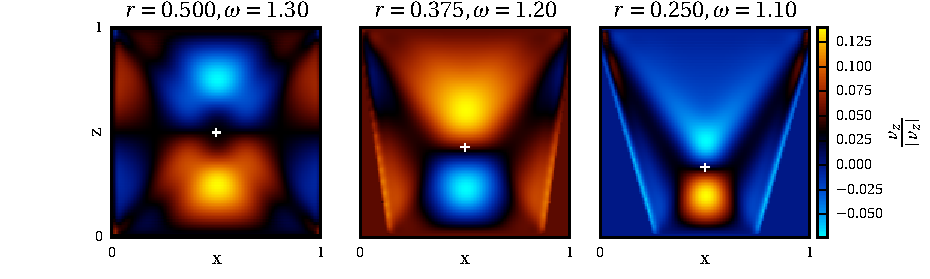
\includegraphics{gfx/cone/transition/phase.pdf}
  \caption{\label{fig:cone:phase}
    Simulation of
  }
\end{figure}

\clearpage

\subsection{Librating Cone with Differing Offsets at the Top}
\subsubsection{Introduction}

A a closure, this section represents the results computed with a new modified setup, which are more in accordance
with the experiment we introduced.
The improvements are based on the results and insights, which were gained from the previous simulations of the librating cone.
We want to adress the  most important points

\begin{itemize}
    \item The radius of the bottom plate of the frustum has a strong influence on
          the reflection of inertial waves.
          Due to the Ekman number of $\Ekman=10^{-4}$ we use, which is one order of magnitude
          above the experiment we assumed that a stronger damping acts on an inertial wave
          at the bottom plate.

    \item As a second point, we want to adress the influence of the offset on top of the cone,
          which has been left out from any discussion so far.
          It can be assumed this offset has a strong influence
          on inertial wave propagation.
          In particular for the intervall $\Theta<\alpha$, where wave super-critical reflection into the top corners occurs.
          In the case where $O=0$, the corners of the cone act as an attractor, as pointed out in figure \ref{cone:img_finalattractor}.
          For small gap sizes it applies that a inertial wave will be damped, in analogy to the bottom gap.
\end{itemize}

As a conlusion a larger gap radius $r$ for the bottom plate, will be introduced.
The exact influence of the offset is unknow, therefore we propose a series of simulations with different offsets.

\begin{figure}[!bp]
      \centering
        \resizebox{0.9\textwidth}{!}{
       \import{gfx/cone//}{comparison.pdf_tex}
      }
      \caption{
          Wave reflection for $o>0$ in the upper edges of the cone (left) and
          an attractor for $o=0$ (right), in the upper edges of the cone.
      \label{cone:img_finalattractor}
      }
\end{figure}

\subsubsection{Setup}

In this setup the radius $r$ is implitciy set by changing the height of the
bottom plate to $h_b=0.375$.  The resulting radius is $r \approx 0.22$.
This is done in order to maintain the constant slope of $\alpha=60$,
which is parallel to an inertial wave for $\omega=1$.
An additional offset is added to the default one,
varying in the range of $h_+ = [0, 0.5]$ with a stepsize of $\Delta h_+ = \nicefrac{1}{5}$.
The complete offset at the top is $O =  (\nicefrac{1}{2})\tan{\nicefrac{\pi}{3}}{2}+ h_+$.
The main simulation parameters are given by

\begin{center}
\vspace*{0.7ex}
\begin{tabular}{c|c|c|c|c|c|c|c }
%\begin{tabular}{p{0.1\linewidth}| p{0.1\linewidth}| p{0.1\linewidth}|  p{0.1\linewidth}| p{0.1\linewidth}| p{0.1\linewidth} }
$\leftarrow h_+\rightarrow$ & $ \leftarrow  \omega \rightarrow $ & $\Delta t$ & $\Delta x$ & $c^2$ & \Ekman  & $l_x, l_y, l_z$ & $T^*_{end}$\\
\hline
$[0,\; 0.5], \Delta h_+ =0.125$ & $[0.2,\; 2], \Delta w = \nicefrac{1}{20}$ & $10^{-5}$ & $\nicefrac{1}{128}$ & 500 & $10^{-4}$  & (1, 1, $1+h_+$) & $\gtrsim100$\\
\end{tabular}
\vspace*{0.7ex}
\end{center}

It should be noted that a higher resolution for the frequency was used compared to the previous simulations.
The total simulation time $T^*_{end.}$ is marked as $\gtrsim 100$, here we want to introduce the modification

\begin{align}
    T_{\text{end.}}^* = \underbrace{\Bigl\lfloor\left(\text{T}_{\text{end}}\frac{\omega}{2\pi}\right)\Bigr\rfloor}_{
        \text{Floor}
        }\frac{2\pi}{\omega} + \frac{2\pi}{\omega}
\end{align}

As a consequence the endtime  of all frequencies, is set to the point where the librating force is crossing zero.
The scenario we want to study from there on is the decay of inertial waves.
To achieve this we continue a simlations with the previously computed endstates and set the libration amplitude $\epsilon$ to zero.
With the use of the modified endtime, we assume all that all intertial waves are
approximately in the same phase with respect to their libration frequency.
The simulation parameters changes according to

\begin{center}
\vspace*{0.7ex}
\begin{tabular}{c|c|c|c}
%\begin{tabular}{p{0.1\linewidth}| p{0.1\linewidth}| p{0.1\linewidth}|  p{0.1\linewidth}| p{0.1\linewidth}| p{0.1\linewidth} }
$\leftarrow h_+ \rightarrow$ & $ \leftarrow  \omega \rightarrow $ & $\epsilon$ & $T_{\text{end}}$\\
\hline
 see \ref{p.xx} & see \ref{p.xx} & 0 & 150\\
\end{tabular}
\vspace*{0.7ex}
\end{center}

For h and w choose specific points as explained in the discussion ( ?)
As a last step we will repeat a part of the simulations for an Ekman number of $\Ekman = 10^{-3}$
-hd simulaiton nachträglich

\clearpage

\subsection{Results}
\subsubsection{Spectrum for the Simulation with Different Offsets}

The results for this simulation are shown in figure \ref{fig:cone:finaltransition}.
On the left side of the plot  the frequency spectrum is shown, the right side illustrates the used geometry.
The height $h_+$ is in descending order, from top to bottom.
Each plot contains two spectra, one for the cone  and the other one for the frustum.
We beginn with a qualitative description of the curves for the frustum.\\
At all heights $h_+$, several resonance modes can be observed. For now we will consider the case where ${h_+=0.25}$.
For this height the largest peaks occur in the spectrum, which are numerated here in decreasing order of the amplitude.\\
The largest mode (\RN{1}) can be observed at a frequency $\omega=1.05$, the amplitude is of the order $5\cdot10^{-4}$.
The second mode (\RN{2}) can be found at $\omega=0.9$ of order $3.7\cdot10^{-4}$, followed by
a possible mode (\RN{3}) at $\omega=0.5$ of order $2.8\cdot10^{-4}$.
On the right side of the spectrum there are two possible small resonances at $\omega=1.7$ and $\omega=1.5$ (\RN{4}, \RN{5}).
For the case $h_+=0.5$  we can see small additional resonances  (\RN{6}) at $\omega=1.8$ and (\RN{7}) at $\omega=0.55$,
the latter is embedded in the slope of the (\RN{3}) mode.
For all peaks (except (\RN{7}), it can be noted, that a lowering of the offset height $h_+$ results
into a shift towards higher frequencies. This can be best seen when looking at the peaks (\RN{1}) and (\RN{2}).\\
Let us now consider the results of the cone.
Above the critical slope $\alpha=\theta$ nearly all resonances are eliminated. One exception is the (\RN{4}) mode for
$h_+=0.5$ and $h_+=0.375$. Another exepction is at the position of the previous (\RN{1}) mode of the frustum.
For $h_+=0.5$ (see \textbf{O}) a small increase in the amplitude can be observed.
On the left side of the critcal slope we can identfiy the (\RN{3})-peak
at the same frequency and same order as for the frustum. To the left side of this point the spectrum for
the cone and the frustum are similar.

\begin{figure}[!bp]
  \centering
  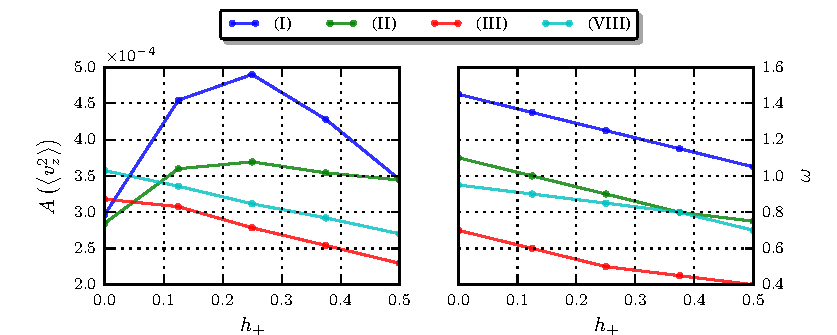
\includegraphics{gfx/cone/final/amp_pos.pdf}
  \caption{
      \label{fig:cone:finalampmax}
    top.
    }
\end{figure}

\begin{figure}[!pt]
  \centering
  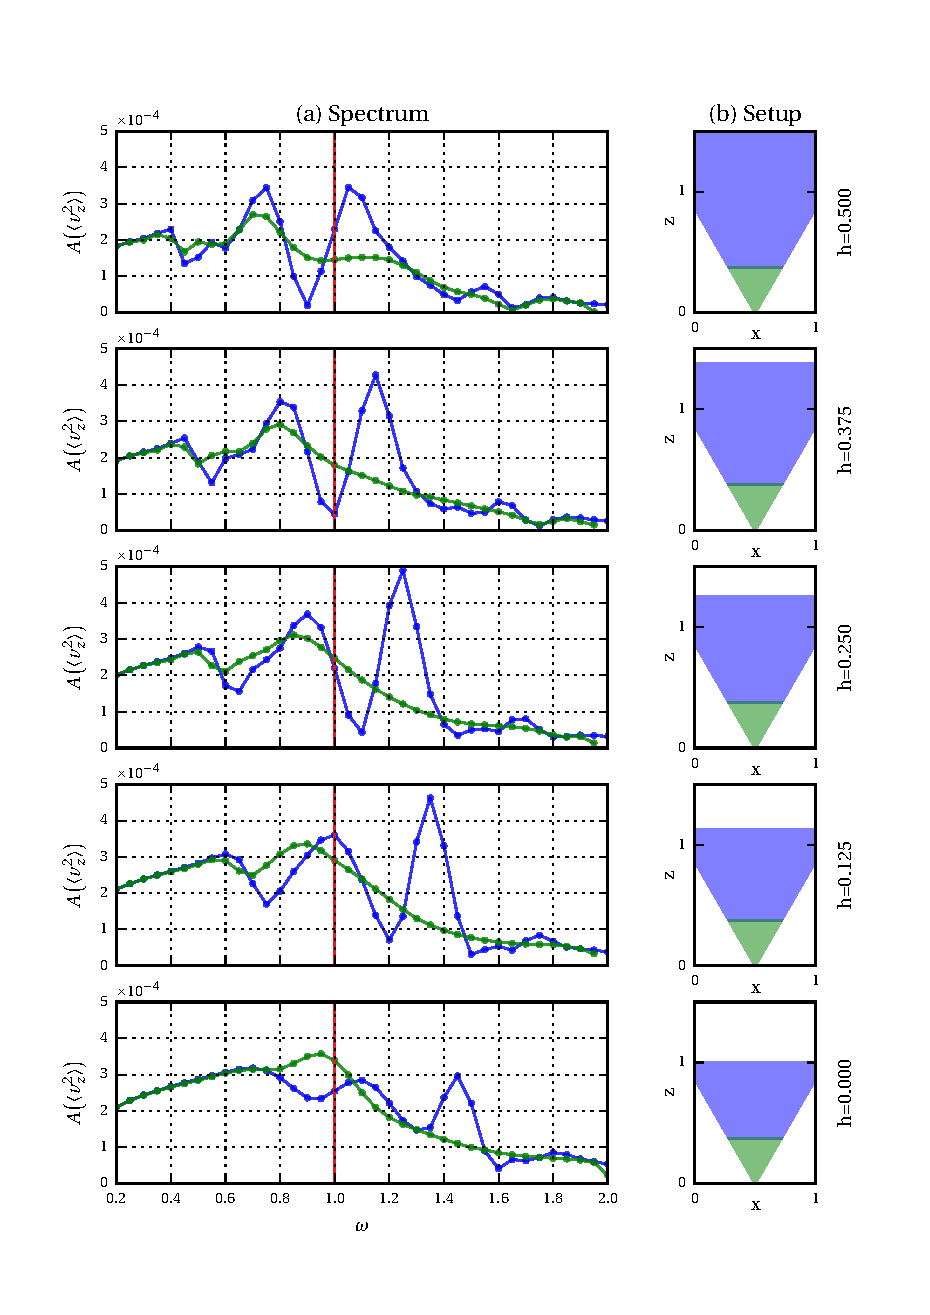
\includegraphics{gfx/cone/final/transition.pdf}
  \caption{
      \label{fig:cone:finaltransition}
    Simulation of a cone (green) and a frustum (blue) for different offsets at the
    top.
    }
\end{figure}
\clearpage

Furthermore at the position of peak (\RN{2}) of the cone, we now see a slightly diminshed mode \RN{8}.
The maximum is at the same frequency at $h_+=0.5$ but diverges slightly with an decrease of the height $h_+$.\\
comparison:
-symetrie h0.5 mode 1 2
-asymertie mode 1 h0.5

-comper cone to frustum
-offset propt to peak shift to left
-amplitude
-plot peak shift

-plot amplitude shift
-discuss plot

qualitative:
-bestimmung maxima und amplituden
-dargestellt in plot ...
- discussion
-anstieg m1 und m2
-abfall m3 und m8
relativ linear abfall für alle moden
-allerdings auflösung dafür nicht gut
-comper cone to frustum
-offset propt to peak shift to left
-amplitude

-plot peak shift
-plot amplitude shift

-discuss plot



\subsubsection{Helicity}

-helicity results shown in figuren..
- global or acc
- nicht so ins detail gehen
- important features
- steigung beim critical slope
- diskutiere bereiche links rechts
- sehr kleine helizität

\subsubsection{Decay rates}

-ablkingraten für maxima ploten und vergleichen den verlauf
-resultate fit schnell gemacht
- positionen erläutern
- ablkingraten dargestellt in figure so und so
- diskussion

\subsubsection{High Resolution Comparison}

\subsubsection{Larger Ekman number}

-test alte ergebnisse evtl erläutern

\clearpage

\subsection{Discussion}

\subsubsection{Spectrum for the Simulation with Different Offsets}

-links von m3 gleiches spectrum bild strahlengang bei m3
-shift geometrie erklärung
-vergleich zylinder mode evlt im paper nachschauen
-gucke animationen alle moden im vergeich beispielbilder  cone/frustom vgl

-fehler 8er mode bild zylinder theorie reibung

\subsubsection{Helicity}

-helicity is sehr klein system ist nicht gut geignet für einen dynamo?
-check fehler berechnung l2 norm

\subsubsection{Decay rates}



-results erstmal machen
-wichtig diskussion turbulenz!

\subsubsection{Larger Ekman number}

\subsubsection{Ray Tracer}


\subsection{Summary}
freeslip besser

In addition to default helicity compuattion, we will also compute

Furthermore we will compute the normalized helicity of the system given by
in the accelerated frame of reference and also for the inertial system with an additional offset in the velocity
given by $\vec{u} = \vec{u}|_{\text{rot.}} + \Omega(t) \times \vec{r}$.
\\


\newpage
\thispagestyle{empty}
\mbox{}

\printbibliography

% \chapter*{Danksagung}

\begin{otherlanguage}{ngerman}
  \thispagestyle{empty}





  \null\vfill
  \noindent
\end{otherlanguage}

\end{document}
